\documentclass[11pt]{article}
%Gummi|061|=)
\usepackage[english]{babel}
\usepackage[utf8]{inputenc}
\usepackage{hyperref}
\usepackage{graphicx}
\usepackage{amsmath}
\usepackage{frontespizio}
\usepackage{subfig}


% this is to have a new page for each section
\usepackage{titlesec}
\newcommand{\sectionbreak}{\clearpage}

%\DeclareMathOperator{\Tr}{Tr}
%\DeclareMathOperator{\Exp}{exp}
\DeclareMathOperator{\Log}{log}
%\DeclareMathOperator{\Det}{det}
\numberwithin{equation}{section}

\title{TITLE TITLE TITLE}
\author{Alberto Botto Poala\\
Advisor Prof. Dr. Friedrich Röpke}
\date{07.03.17}
\begin{document}
\begin{titlepage}
\begin{center}

% Upper part of the page. The '~' is needed because \\
% only works if a paragraph has started.
% to set spelling in Vim type :setlocal spell spelllang=en_us

\textsc{\LARGE Universität Heidelberg}\\[1.8cm]

\textsc{\Large Master Thesis}\\[0.5cm]

% Title

{ \huge \bfseries title title title title title \\[0.5cm] }



% Author and supervisor
\begin{minipage}{0.4\textwidth}
\begin{flushleft} \large
\emph{Candidate}\\
Alberto \textsc{Botto Poala}
\end{flushleft}
\end{minipage}
\begin{minipage}{0.4\textwidth}
\begin{flushright} \large
\emph{Advison Professor} \\
Prof. Friedrich \textsc{Röpke}
\end{flushright}
\end{minipage}

\vfill

% Bottom of the page
{07.03.17}

\end{center}
\end{titlepage}

\tableofcontents
\maketitle

%%%%%%%%%%%%%%%%%%%%%%%%%%%%%%%%%%%%%%%%%%%%%%%%%%%%%%%%%%%%%%%%%%%%%%%%%%%%%%%%%%%%%%%%%
% SECTION INTRODUCTION
%%%%%%%%%%%%%%%%%%%%%%%%%%%%%%%%%%%%%%%%%%%%%%%%%%%%%%%%%%%%%%%%%%%%%%%%%%%%%%%%%%%%%%%%%

\section{Introduction}
Nature in known for having three mechanisms to transport heat.  \\
The first one is through \textbf{heat conduction}. If we suppose to have two identical bricks of iron but at two different temperatures and we could look at the atomic scale, the only difference we would notice is that the atoms of the warmer brick shake more. To say it in a more rigorous way, their mean kinetic energy (with a randomized velocity) is higher, hence the thermal energy of the brick. If we imagine to put the two bricks in contact, the atoms of the warmer would start to hit and bounce on the atoms of the colder, transfering thermal energy (or heat) from the one to the other, until they reach a situation of equilibrium. This is of course the \textbf{Principle Zero of Thermodynamics}. \\
The second one is \textbf{radiation}. Every object with a non-zero temperature emits a black body radiation, as long as atomic bounds are complex enougth in order to allow the application fo Boltzman statistics for the energetic distribution of electrons (but this is true for objects that have a number of atoms in the order of the Avogadro Number, and even far less). This allows a body to lose thermal energy over time through emission of elecromagnetic radiation. This is the mechanism through which Earth and other planets re-emit the radiation received by the Sun and reach thermodinamic equilibrium (it cannot happen through conduction, since this would require that molecules in the atmosphere would transfer their thermal energy to molecules or atoms in space, which are too rarefied to allow this). \\
The third mechanism, which is the topic of this Thesis, is \textbf{convection}. When we have a fluid stratification like in the atmosphere, if certain thermodinamyc condition are fuilfilled, this might become unstable in certain regions and give rise to macroscopic ascending and descending blobs, that later decay to smaller scale blobs and finally into turbulence. This enables a very effivcient transfer of quantities such as heat and chemical composition through different layers of the fluid stratification. \\
A \textit{Cumulonimbus}, the typical cloud of thunderstorms, is a perfect example of such phenomenon. They seldom reach an altitude higher that ten thousand meters because thermodynamical conditions for convection are generally prohibitive in these regions of the atmosphere. Nevertheless when a convective blob hits the stable layer, two fenomena happen. First of all its turbulent motion erodes mass from it and over time the convective boundary moves upward. Second of all the hit of the blob imprints an internal mode in the stable layer. These two are the reasons for which planes avoid flying not only into tunderstorms but also above them, because they expect to find turbulence. \\
This phenomena happen also in stellar interia. A convective region over time accrets mass from the stable one, mixing energy and chemical composition (and hence affecting nuclear reaction rates) and imprints internal modes that can be observed on stellar surfaces (the field that study this phenomenon is asterosismeology, that relies on data of space observatory such as \textit{KEPLER}). It is therefore of fundamental importance to understand the dynamic of the convective boundary and the \textbf{Convective Boundary Mixing} (CBM) problem, in order to properly understand stellar evolution. This is the ultimate goal of this work.
%%%%%%%%%%%%%%%%%%%%%%%%%%%%%%%%%%%%%%%%%%%%%%%%%%%%%%%%%%%%%%%%%%%%%%%%%%%%%%%%%%%%%%%%%
% SECTION UNDERLYING PHYSICS
%%%%%%%%%%%%%%%%%%%%%%%%%%%%%%%%%%%%%%%%%%%%%%%%%%%%%%%%%%%%%%%%%%%%%%%%%%%%%%%%%%%%%%%%%

\section{Underlying Physics}
\subsection{Hydrodynamics}
\subsubsection{Derivation of the Equations of Ideal Hydrodynamics}
As all the most beautiful and successful laws of Physics, Hydrodynamics is derived from some conserved quantities. \\
Let's consider for instance a monoatomic gas in a box. A fundamental assumption in ideal hydrodynamics is that the mean free path of particles is infinitesimal. Particles might be spatially equally distributed (like in a bottle) or might not (maybe because the box is so big that we get a stratification like in the atmosphere). Same concempt holds for the velocity distribution, it might be Maxwellian or it might not be. 
In any case we can define the \textbf{distribution function in phase space} $f( \vec{x^{\mu}}, \vec{p^{\mu}})$ such that

$$N=\int \ d^4x \ d^4p \ f( x^{\mu}, p^{\mu}) \  \delta_D[(p^0)^2-\vec{p}^2+m^2c^2] \  \Theta(p^0)$$ 
 where $N$ is the total number of particle, $\delta_D$ is the Dirac $\delta$ function that selects in the integrations only the hypersurfaces physically allowed by the energy-momentum relation of General Relativity, and finally $\Theta$ makes sure that we are taking into account only positive momenta. 
Keeping this in mind, we can define the first and second momentum of our distribution function

\begin{align}
J^{\alpha}= c \int \frac{dp^3}{E} \ f( x^{\mu}, p^{\mu}) p^{\alpha}  &&   T^{\alpha \beta}= c \int \frac{dp^3}{E} \ f( x^{\mu}, p^{\mu}) p^{\alpha}p^{\beta}  
\end{align}
 
namely the \textbf{current density} $J$ and the \textbf{energy-momentum tensor} $T$. Carrying out the calculation the components read 


\[
  J= \frac{n(t,\vec{x})}{c}
  \begin{pmatrix}
    c \\
    \left< \dot{x} \right> \\
    \left< \dot{y} \right> \\
    \left< \dot{z} \right> \\
  \end{pmatrix}\quad
  T= \rho(t,\vec{x})
  \begin{pmatrix}
    c^2 \left< \gamma \right> & c \left< \gamma \dot{x} \right> &  c \left< \gamma \dot{y} \right> & c \left< \gamma \dot{z} \right> \\
     c \left< \gamma \dot{x} \right> & \left< \gamma \dot{x}^2 \right> &  \left< \gamma \dot{x}y \right> &  \left< \gamma \dot{x} \dot{z} \right>  \\
     c \left< \gamma \dot{y} \right> &  \left< \gamma \dot{y} \dot{x} \right>&  \left< \gamma \dot{y}^2 \right> &  \left< \gamma \dot{y} \dot{z} \right>  \\
     c \left< \gamma \dot{z} \right> &  \left< \gamma \dot{z}\dot{x} \right>& \left< \gamma \dot{z}\dot{y} \right> &  \left< \gamma \dot{z}^2 \right> 
  \end{pmatrix}
\]

where $n(t, \vec{x})$ is the number density, $c$ the speed of light,  $\left< a(t,\vec{x}) \right>$ means the average of the quantity $a$ over time and space in a neighborhood of $(t, \vec{x})$, $\gamma$ is the well known general relativistic parameter.\\
By integrating the first and second momentum of Boltzmann Equation, one could show that $J$ and $T$ are divergenceless, meaning in the non-relativistic case
\begin{align}
\frac{\partial }{\partial^{\mu}}J^{\mu}=0 && \frac{\partial }{\partial^{\mu}}T^{\mu \nu}=0 \  \  \forall \nu =0,..,3 
\end{align}
This means that if we strike $J$ and $T$ with the operator $(c^{-1}\partial_t,\partial_x,\partial_y,\partial_z)$ from upside down we equal zero. Doing so with the density current we obtain the \textbf{continuity equation}
\begin{equation} \label{cont}
\partial_t \rho + \vec\nabla \cdot (\rho \vec{v})=0
\end{equation}
We then apply the same procedure to the energy-momentum tensor.\\
We might choose to do it in the first column ($\nu=0$), and that would lead us to the \textbf{energy conservation equation}
\begin{equation} \label{consen}
\partial_t \epsilon + \vec \nabla \cdot (\epsilon \vec{v}) + P\vec \nabla \cdot \vec{v}=0
\end{equation}
where $\epsilon$ is the internal energy and $P$ the pressure. These two variables, that were not esplicitally included in $T$, arise naturally by splitting up the microscopic velocity of the fluid $\left <  \dot{x} \right >$ into a mean macroscopic velocity $\vec{v}$ and a random velocity $\vec{u}$ in the neighborhood of the mean one. 
$$\left <  \dot{x} \right >= \vec{v}  +  \vec{u} $$
and recalling that 
$$\epsilon = \frac{\rho}{2} \left <  u^2 \right > = \frac{3}{2} n k_B T= \frac{P}{2}$$
When we strike on the other three columns of $T$, we obtain the \textbf{momentum conservation equations} for the three spatial dimensions.
\begin{equation} \label{euler}
\partial_t \vec{v} + (\vec{v} \cdot \vec \nabla) \vec{v} + \frac{\vec \nabla P}{\rho}=0
\end{equation}
These last three are often called \textbf{Euler equations}. \\
Note that the operator on the left hand side is nothing but the total time derivative
$$
\partial_t + \vec{v} \cdot \vec \nabla = \frac{d}{dt}
$$
so what we are actually writing is Newton's equation per unit volume
$$
\rho \vec{a} = \vec \nabla P
$$
In case other macroscopic forces like gravity are present, we simply add them on the right hand side as we would do in Classical Mechanics. \\
So far we have obtained 5 equations in 6 unknowns, namely the internal energy $\epsilon$, the momentum $\vec{p}$, the pressure $P$ and the density $\rho$. If we want to have at least a chance of integrating the system we're missing one equation, the \textbf{equation of state}, that relates the thermodynamic variables.

\subsubsection{Viscous Hydrodynamics}

As stated at the beginning of the previous subsection, one fundamental assumption of ideal Hydrodynamics is that particles have an infinitesimal mean free path. What actually happens in nature might be very different. Particle have a finite mean free path, and hence they can transport local property all through the fluid by diffusion: transport of energy generates heat conduction, transport of momentum friction. The consequence is that we end up with one additional term in the energy-momentum tensor representing the diffusive processes
$$
T^{ij} \to T^{ij} + T^{ij}_d 
$$

The density current remains unchanged (and hence continuity equation) because mass is always conserved. As in the previous subsection, the new energy-momentum tensor needs to be struck with $\nabla$ and set equal to zero in order to obtain our modified equations in the viscous case. We will not carry out all the calculations, rather simply quote the result for the voscous versions \ref{consen} and \ref{euler}. \\
The new energy conservation equation reads
$$
\partial_t \epsilon + \vec \nabla \cdot (\epsilon \vec{v}) + P \vec \nabla \cdot \vec{v} = \vec \nabla \cdot (k \vec \nabla T) + v_{ij} T_d^{ij} 
$$
where $v_{ij}$ is the symmetrised velocity gradient tensor
$$
v_{ij} = \frac{1}{2}(\partial_i v_j + \partial_j v_i)
$$
This equation shows that the internal energy in a certain region of the fluid can change either if there is a temperature gradient or if the fluid is moving with a velocity field with a non vanishing symmetrised gradient (non solid body rotation like) because of friction.
The new momentum conservation equations read
$$
\rho \left( \partial_t + \vec{v} \cdot \vec \nabla \right) v^j+\partial^jP = \eta \vec \nabla^2v^j + \left( \xi + \frac{\eta}{3} \right) \partial^j \vec \nabla \cdot \vec{v}
$$
These are often called \textbf{Navier-Stokes Equations}, and thoroughly show the nonlinearity of Hydrodynamic.

\subsubsection{Hydrostatic Equilibrium in Stars}
We shall now consider the static configuration of \ref{euler} with gravitational potential. This reads
\begin{equation} \label{hystat}
	\vec \nabla P = - \rho \vec \nabla \Phi
\end{equation}
This shows that the pressure stratification is adjusted only by the shape of gravity. We can say more by taking the curl of this equation and we get
$$
\vec \nabla \rho \times  \vec \nabla \Phi =0
$$
which shows that the gradient of the gravitational potential and of the density are parallel. Surfaces of constant density are surfaces of constant gravitational potential.\\
It is known from Classical Mechanics that if we are given a spherically symmetric matter distribution, the gravitational acceleration is $g=Gm/r^2$ which leads to
\begin{equation}\label{2.4}
	\frac{\partial P}{\partial r}= - \frac{G m}{r^2} \rho
\end{equation}
The general approach to find the relation betwen the pressure and the density consists in taking the divergence of \ref{hystat} and substituting Poisson equation 
$$
\vec \nabla \cdot \left ( \frac{\vec \nabla P}{\rho} \right ) = - 4 \pi G \rho 
$$
This equation can be solved only if an equation of state is provided. For instance if we choose a polytropic equation of state (which means that the pressure is a function of the density only and not of the temperature) we obtain the \textbf{Lane-Emden Equation} that allows stable solutions for adiabatic indices up to $4/3$ only. This EoS is used for instance for modeling white dwarfs, where the pressure doesn't depend on the temperature. \\ 

\subsection{Transport of Energy by Radiation}
In deep interia of stars energy in generated through nuclear reactions. In the Sun for instance basically all the energy is provided by the so called p-p chain, while just a little fraction by virialization. Because temperature is of the order of $10^9 K$, thermal motions allow protons to overcome the electrostatic potential barriers and interact through the nuclear force, giving rise to the reaction
\begin{equation}\label{ppchain}
	6 \mathrm{H}^1 \to \mathrm{He}^4_2 + 2 \mathrm{H}^1 + 2 \gamma + 2 \nu
\end{equation}
where on the right hand side we have photons and neutrinos, that carry energy away. \\
Neutrinos, interacting only via the weak force, have a very low cross section and hence leave the core of the sun without scattering, draining energy very efficiently. We need to take into consideration very massive systems like Core Collapse Supernovae and Neutron Stars in order to see a tangible interaction between the neutrino flux and matter. Actually these astronomic objects are excellent neutrino laboratories gently provided by Nature. \\
Photons instead, interacting electromagnetically, scatter multiple times before reaching the \textit{photosphere}, the region where statistically they scatter for the last time before ending up in our eyes or our telescopes. \\
Let's now make a rough estimate of the mean free path of a photon in the sun. 
\begin{equation}\label{mfp}
	l_{p,p}=\frac{1}{k \rho}
\end{equation}
where $k$ is the mean cross section (averaged over all frequencies) per unit mass. For ionized hydrogen in stellar medium a rough average is $1 \ cm^2/g$. The average density of the sun is $\bar\rho_{\odot}=3M_{\odot}/4 \pi R_{\odot}^3= 1.4 \mathrm{g /cm}^3$. \\
Plugging in the numbers we get $\bar l_{p,p \odot}=2 \  \mathrm{cm}$. \\
At this point we need to answer a fundamental question: does two sequential scatterings happen at thermodinamic equilibrium? In other words when one photon scatter, and then scatters again a few millimeters or centimeters away, does it encounter the same thermodinamic conditions? In order to evaluate that, let's consider the mean temperature gradient between the center of the sun and the photosphere
$$
\frac{\Delta T}{\Delta r} = \frac{10^7 \ \mathrm{K}-10^4  \ \mathrm{K}}{R_{\odot}} \simeq 1.4 \times 10^{-4} \  \mathrm{K} \ \mathrm{cm} ^{-1}
$$
which means that after $2 \mathrm{cm}$ on the radial direction a photon sees a difference in temperature of $\Delta T = l_{p,p} \times 1.4 \times 10^{-4}  \  \mathrm{K} \ \mathrm{cm} ^{-1}= 3 \times 10^{-4} \  \mathrm{K}$. The relative difference of radiation energy density can be easly computed since $u \sim T^4$, hence in the center of the sun $\Delta u/u=4 \Delta T / T \sim 10^{-10}$: between two scatterings a photon is in \textbf{Local Thermodynamic Equilibrium} (LTE). This little anisotropy that we neglect is the actual cause of the luminosity of the sun, because it generates a non-vanishing net flux.
\subsubsection{Diffusion of radiative energy}
We have seen that the mean free path $l_{p,p}$ of photons is much smaller that the characteristic length of our physical system, hence we are allowed to treat the scattering processes statistically. This leads us to describe energy transfer as a diffusion process. \\
The diffusive flux $j$ of a certain species of particles (number of particles migrating per unit area and unit time) is given by
\begin{equation}\label{diffusion}
	\vec  j=-D \nabla n
\end{equation}
where $n$ is the species density. $D$ is the diffusion coefficient
\begin{equation}
	D =\frac{1}{3} v l_{p}
\end{equation}
function of the mean free path and of the mean velocity. What we are actually intrested in is not the diffusive flux of the particles $j$, but rahter in the diffusive flux of their energy $\vec F$. The density needs to be substituted with the energy density $u=aT^4$, $\bar v$ with $c$ and $l_p$ with $l_{p,p}$. $a$ is the radiation density constant. If we assume spherical symmetry the gradient of $u$ is simply the radial component
\begin{equation}
	\frac{\partial u}{\partial r} = 4  a  T^3   \frac{\partial T}{\partial r}
\end{equation}
So recalling \ref{diffusion} we have immediately that
\begin{equation}
	F=-\frac{4ac}{3}\frac{T^3}{k \rho} \frac{\partial T}{\partial r}
\end{equation}
which can be written down in a more compact way as 
\begin{equation}
	\vec F = - k_{rad} \nabla T
\end{equation}
after having properly defined $k_{rad}$ as the conduction coefficient. Now we use the well known relation between luminosity and flux and solve it for the temperature gradient
\begin{equation}
	\frac{\partial T}{\partial r}= - \frac{3}{16 \pi a c}\frac{k \rho l}{r^2 T^3}
\end{equation}
which in lagrangian coordinate reads
\begin{equation}\label{partialTpartialm}
	\frac{\partial T}{\partial m}= - \frac{3}{64 \pi^2 a c}\frac{k l}{r^4 T^3}
\end{equation}
We shall never forget the assumptions we did when deriving this equation, namely the LTE. When we approach the photosphere for instance the density decreases, the mean free path increases, and two scattering events happen so far away that LTE doesn't hold any longer. In this case radiation transport is no more a diffusive process. \\ 
Another form of heat transfer is conduction, but in stellar physics it becomes relevant only in cores of red giants or white dwarfs and it is fully neglected in our simulations.
\subsubsection{The astrophysical $\nabla$}
Assuming hydrostatic equilibrium we can now divide \ref{partialTpartialm} by REF and obtain
\begin{equation}
	\frac{\partial T/\partial m}{\partial P / \partial m} = \frac{3}{16 \pi a c G} \frac{k l}{m T^3}
\end{equation}
This is nothing but the derivative of the temperature with respect to the pressure, that increasing monotonically inward is representative of the radious. We furthermore rewrite this quantity as
\begin{equation}\label{nablarad}
	\nabla_{\mathrm{rad}} = \left( \frac{d \ln T}{d \ln P}  \right)_{\mathrm{rad}}= \frac{3}{16 \pi a c G} \frac{k l P}{m T^4}
\end{equation}
This quantity will be of fundamental importance when we will discuss convective stability. Recall that we took into account only radiative transfer, but defining $k$ properly we could take into account also heat conduction.
\subsection{Fundamental Equations of Stellar Structure}
At this point we are able to write down a system of equation that we will call \textbf{fundamental equations of stellar structure}, which describe an oversimplified thus very useful model. This will hold in a static, stable and spherically symmetric case.\\

\textbf{Mass continuity} \\
Here $m(r)$ is the mass contained inside the sphere of radius $r$
\begin{equation}\label{masscons}
	\frac{dm}{dr}=4 \pi r^2 \rho
\end{equation}

\textbf{Hydrostatic equilibrium} \\
We have already encountered the hydrostatic equilibrium equation
\begin{equation}\label{hydroeq}
	\frac{dP}{dr}= - \frac{G m(r)}{r^2} \rho
\end{equation}

\textbf{Equation of State} \\
So far we have written down two equations in three variables, namely $m$, $\rho$, and $P$. If we want to have at lest a chance to solve them we need another equation, namely the equation of state. Possible choices are:
\begin{itemize}
	\item $\rho=const$ this would be the case for liquids.
	\item $P\propto \rho^\gamma$ i. e. the density and pressure are not a function of the temperature. This is the case, as already stated in the previous section for white dwarfs and leads to the Lane-Edmen equation and its solutions.
	\item $P=\frac{\mu}{R}\frac{P}{T}$ the equation of state for perfect gases and it's the case for the sun. It has the inconvenient that it introduces another variable, namely the temperature $T$, and hence it doesn't solve our original problem. We need at least another equation to solve the system. 
\end{itemize}

\textbf{Energy conservation} \\
In case we have an energy source (such as nuclear reactions), this needs to be conserved
\begin{equation}\label{energycons}
	\frac{dL}{dr} = 4 \pi r^2 \epsilon
\end{equation}

\textbf{Temperature gradient} \\
Of crucial importance to understand convection will be the following equation for the astropysical nabla
\begin{equation}\label{energytransfer}
\frac{d T}{d r} = - \frac{T }{P} G m \rho\nabla
\end{equation}


\subsection{Convection}
Until now we have assumed a perfect spherical symmetry, meaning that all dynamical and thermodynamical quantities were a function of the radius only. Obviously this is not a realistic case. For a number of reasons stars have small perturbations, that may eventually grow and give rise to macroscopic phenomena. A classic example is convection.\\
We are relaxing the spherically symmetric case, but this doesn't mean that our fundamental equations of stellar structure are useless. As explained in the introduction, if we could section stars we would see that convection appears in concentric regions, hence  we can still treat the problem as spherically symmetric defining dynamycam and thermodynamical quantities as averages on a proper region. \\
We shall now understand when, given thermodynamic variables, we are dealing with a dynamically stable or unstable layer.


\subsubsection{Dynamical instability}
Let's consider a perfect density stratification like the one in a star or in the atmosphere and let's break the symmetry of the system by adding a little perturbation in the termodynamic variables. For any given quantity $A(r, \theta)$ (from now on $A_e$, because it's a function of the mass element we are considering), we compute $A_s$ (which is an average at given $r$ on the surrounding material). We shall furthermore assume that the fluid moves adiabatically, thus the timescale for heating transfer is much smaller than the timescale for convection turnover. \\
We define a local property of the fluid 
$$
DA=A_e - A_s
$$
For instance we could imagine that a little region of a star is slightly hotter than the surroundings, hence we have in that region $DT > 0$. Note that because of the assumption we have made $DP=0$ always, because when these is a pressure spike, the gas expands at the sound velocity $c_s$ which is way higher than the low hydro regime we observe in stellar inertia.\\
If we have a $DT>0$, since in a perfect gas the equation of state reads $\rho \sim P/T$, we obtain $D \rho < 0$. With a lower density, that mass element will be lifted by buoyancy force. In a non adiabatic workframe it might happen that heat is exchanged so quickly that temperature differences vanish immediately, but we assumed adiabatic processes. The question we are trying to answer is if the mass element, after a little upward movement, will still be buoyant and give rise to macroscopic convection, or if it will bounce back. The answer lyes obviously in the temperature gradient, i. e. if once lifted of a little bit the new $DT$ will still be in favor to buoy it to the next layer, and so on. \\
Let's approach the problem from another point of view. Let's assume that we have a stable layer without perturbations, and we lift a mass element upward of $\Delta r$. The density difference now is
\begin{equation}\label{displacment}
D \rho = \left [  \left( \frac{d \rho}{d r} \right)_e - \left( \frac{d \rho}{d r} \right)_s   \right ] \Delta r
\end{equation}
where the first derivative tells us how much the density of the mass element changes when lifted, the second one tells us how the surrounding density changes along the radial direction. \\
We call the buoyancy force per unit volume 
$$
f_b=- g \ D \rho
$$
which points upward if $D \rho < 0$, which is the unstable configuration. If instead $D \rho > 0$ the mass element sinks back to its original position and no macroscopic motion appears. As a consequence $D \rho<0$ is our \textbf{condition for stability}.\\
The problem with this criterion is that very often the density gradient is not known, since it does not appear in the fundamental equations for stellar structure. In order to proceed let's turn our gradient in spacial coordinate into a gradient in thermodynamic coordinates. As previously stated, our transformations are adiabatic, hence no exchange of energy occurs. This is very close to reality for stellar intertia. To begin let's write down the equation of state $\rho = \rho (P, T, \mu)$ in a differential form
\begin{equation}\label{EoSdiff}
	\frac{d \rho}{\rho} = \alpha \frac{d P}{P} - \delta \frac{d T}{T} + \phi \frac{d \mu}{\mu}
\end{equation}
where $d \mu$ represents the change in the chemical composition, including ionization processes. \\
Substituting REF in REF we obtain
\begin{equation}
	\left (\frac{\alpha}{P} \frac{dp}{dr}\right )_e - \left ( \frac{\delta}{T}\frac{dT}{dr}\right )_e -  \left (\frac{\alpha}{P} \frac{dp}{dr}\right )_s +  \left ( \frac{\delta}{T}\frac{dT}{dr}\right )_s -  \left ( \frac{\phi}{\mu}\frac{d \mu}{\mu dr}\right )_s>0 
\end{equation}
The two terms containing the pressure gradient cancel each other out because as previously stated $DP=0$. Let's multiply the remaining terms by the so calles \textbf{pressure scale height} $H_P$
\begin{equation}\label{scaleheight}
	H_P=-\frac{dr}{d \ln P}= - P \frac{dr}{dP}
\end{equation}
$H_P$ has the dimension of a length, being the characteristic distance over which the pressure changes.
We finally obtain our condition for stability
\begin{equation}\label{criterionstab}
	\left (   \frac{d \ln T}{d \ln P}    \right )_s <  \left (   \frac{d \ln T}{d \ln P}   \right )_e +  \frac{\phi}{\mu} \left (   \frac{d \ln \mu}{d \ln P}    \right )_s
\end{equation}
We have already encountered the first term which is $\nabla_{rad}$ of \ref{nablarad}.
Let's define two new quantities
\begin{equation}\label{nablas}
	\nabla_{e} = \left (  \frac{d \ln T}{d \ln P}   \right )_e \  \nabla_{\mu} = \left (  \frac{d \ln \mu}{d \ln P}   \right )_s
\end{equation}
Recall that since pressure is always decreasing at increasing radius we can measure the temperature as a function of the pressure, and hence its gradient. Furthermore, since our mass element buoys adiabatically, we call $\nabla_e=\nabla_{\mathrm{ad}}$. 
With this new notation we can write down our stability criterion in a more compact way as
\begin{equation}\label{stabcritcomp}
	\nabla_{\mathrm{rad}} < \nabla_{\mathrm{ad}} + \frac{\phi}{\delta} \nabla_{\mu}
\end{equation}
and obtain the \textbf{Ledoux criterion}. \\
In our simulations we used a monoatomic ideal gas equation of state, hence $\nabla_{\mu}=0$.  What we obtain is the \textbf{Schwarzschild criterion} for dynamic stability
\begin{equation}\label{schwarzschild}
	\nabla_{\mathrm{rad}}<\nabla_{\mathrm{ad}}
\end{equation}
If the left hand side is bigger than the right hand side, it means that our stratification is not able to transport all the energy generated only through radiation, and it is hence required to rely on convection. \\
Note that since now we simply have found a stability criterion, but we don't know anything about the convection that will arise. In the next section we will try to quantify it, especially we need to know how much energy is transported from one layer to the other in order to map this result in 1D simulations of stellar evolution.

\subsection{Mixing length theory}
A fundamental problem in Stellar Astrophysics is to understand how much energy is transported by convection. Before the era of Computational Physics, when only analytics solutions were available, the most common tool used to model convective energy trasnport was the so called \textbf{mixing length theory}. \\
The total energy flux $l/4 \pi r^2$ at given radius is given by the radiative flux $F_{\mathrm{rad}}$ (which may also include the conductive flux), and the convective flux $F_{\mathrm{con}}$. Their summ is according to \label{nablarad} what defines the $\nabla_{\mathrm{rad}}$ that would be necessary to transport away all the energy.
\begin{equation}\label{7.1}
F_{\mathrm{rad}}+ F_{\mathrm{con}}= \frac{4 a c G T^4 m }{3 k P r^2} \nabla_{\mathrm{rad}}
\end{equation}
But part of it is ultimately trasnported by convection, at the most $\nabla_{\mathrm{rad}}$ can equal $\nabla$. 
\begin{equation}\label{7.2}
F_{\mathrm{rad}}= \frac{4 a c G T^4 m}{3 k P r^2} \nabla
\end{equation}
In order to quantify then $F_{\mathrm{con}}$, let's consider a blob with a $DT$ over its surroundings. Its motion will be mainly radial wich a velocity $v$ and with $DP=0$ for reasons already explained. We can write down the energy flux as
\begin{equation}\label{fconv}
	F_{\mathrm{con}}=\rho  v  c_P  DT
\end{equation}
Of course we should average $v$ and $DT$ over an imaginary sphere and hence obtain an equation that holds statistically over the solid angle at a given radius and not locally. One can tell since now the approximations and limits of this theory. \\
Bulbs have an initial velocity that equals zero, and the same holds for $DT$. Over time it will migrate of a discance $l_m$, namely the \textit{mixing length} before dissolving via turbulent cascade. This means that on average a bulb will move of a distance $l_m/2$ where it accelerates, and of another $l_m/2$ where it decelerates of the same amount to stop at the end of the convective zone. Bulbs will definitelly also change shape during the migration, which makes it pretty difficult to strictly define temperature and velocity, but in a very rough approximation we claim that
\begin{equation}
	\frac{DT}{T}=\frac{1}{T}\frac{\partial (DT)}{\partial r} \frac{l_m}{2}=(\nabla-\nabla_e)\frac{l_m}{2}\frac{1}{H_P}
\end{equation}
which is simply a taylor espansion to determine $DT$ after $l_m/2$. Recall that the buoyancy force per unit mass is $f_b=-g \cdot D \rho / \rho$ and that $D \rho / \rho is - \delta D T / T$. Let's pretend on average that half of this force acted on the blob during its migration of $l_m$, hence the work done is
\begin{equation}\label{7.6}
	\frac{1}{2} k_r \frac{l_m}{2}=g \delta (\nabla - \nabla_e)\frac{l_m^2}{8 H_P}
\end{equation}
Let's furthermore suppose that only half of this work ends up in kinetc energy, because the other half has to go in the work necessary for moving the surroundings. Then the average velocity of an element half way is
\begin{equation}
	v^2=g \delta (\nabla - \nabla_e)\frac{l_m^2}{8 H_p}
\end{equation}
and plugging this result into \label{fconv}
\begin{equation}
F_{\mathrm{con}}= \rho c_P T \sqrt{g \delta} \frac{L^2_m}{4\sqrt{2}}H_P^{-3/2} (\nabla-\nabla_e)^{3/2}
\end{equation}
Now let's consider a sphere of diameter $d$ slightly hotter than the surrounding and moving radially with velocity $v$. It will lose energy because of radiative processes and because of the adiabatic expansion. The energy lost in time due to the first proces is
\begin{equation}
\left (\frac{d E}{d t}  \right )_{\mathrm{rad}} = \frac{8 a c T^3}{3 k \rho} DT \frac{S}{D}
\end{equation}
hence the drop in temperautre per unit length travelled radially taking into account both processes is
\begin{equation}\label{7.7}
	\left (  \frac{d T}{d r }   \right )_e = \left(  \frac{dT}{d r }   \right )_{\mathrm{rad}} - \frac{\left( d E / dt \right)_{\mathrm{rad}} }{\rho V c_P v}
\end{equation}
Which multuplied by $H_P/T$ gives
\begin{equation}
\nabla_e - \nabla_{\mathrm{ad}} =  \frac{\left( dE/dt \right)_{ \mathrm{rad} } H_P}{\rho V c_P v T}
\end{equation}
Plugging in the expression that we derived for $(dE/dt)_{\mathrm{rad}}$ and taking an average for $DT$, we are left with an equation that contains a "form factor" $l_m S/Vd$ that for a sphere should of course be $6/l_m$. In the literature it's often used instead $9/2l_m$ and this brings us to
\begin{equation}\label{7.11}
\frac{\nabla_e - \nabla_{\mathrm{ad}}}{\nabla - \nabla_e} = \frac{6acT^3}{k \rho c_P l_m v}
\end{equation}
We finally obtained five equations(\ref{7.1}, \ref{7.2}, \ref{7.6}, \ref{7.7}, \ref{7.11}) in five variables ($F_{\mathrm{rad}}$, $F_{\mathrm{con}}$, $v$, $\nabla_e$, $\nabla$). Note that the mixing length $l_m$ is not one of those variables, and hence is a free parameter for which we have to assume a value. \\
Although the mixing length theory has been used extensively in 1D stellar evolution, in many occasions it has been proven unsuccesfull, especially because of the uncertanties about the parameters. Thanks to the raise of computational resources over the last decade, atmospheric scientists and astrophysicists were able to run 2D and 3D Hydro simulations and approach the problem more heuristically. They concluded that the controlling parameter for the boundary migration could be the \textbf{bulk-Richardson number}, which is the topic of the next section.  


\subsubsection{Bulk-Richardson Number}

So far we got to the point where we have a convective layer and a stable layer above or beneath it. What happens over time is that the convective boundary accrets mass from the stable layer by ingestion, because turbulent eddies capture stable fluid that is consequentially dragged and entrained in the turbulent layer. A fundamental problem in stellar evolution is to understand the dynamics of this boundary: which is its velocity (if we are in an eulerian workframe), or how much mass from the stable layer is entrained in unit time (in a lagrangian workframe).\\
One fo the methods used to model the migration is the \textbf{Bulk-Richardson number}
\begin{equation}\label{bulkrichardson}
	\mathrm{Ri}_{B}=\frac{\Delta b L}{\sigma^2}
\end{equation}
which is a dimensionelss parameter that compares the strenth of the boundary to the one of the turbulence. $L$ is the length scale of the turbulence (which is of course model dependent), $\sigma$ is the rms of its velocity, $\Delta b$ is the buoyancy jump between unstable and stable layer. This is defined by considering the \textbf{Brunt-Väisääla frequency} 
\begin{equation}
	N^2(r)=-g \left (  \frac{\partial \ln \rho}{\partial r} -  \frac{\partial \ln \rho}{\partial r} \Big|_{s}  \right )
\end{equation}
and integrating it over the boundary
\begin{equation}
	\Delta b = \int_{r_i}^{r_f} N^2 dr
\end{equation}
Of course we need a proper definition of the boundary limits $r_i$ and $r_f$, hence also $\Delta b$ is model dependent. \\
Let's furthermore define the \textbf{entrainment coefficient} $E$ as the boundary migration speed $u_b$ over the turbulence rms $\sigma$. Previous works have found that
\begin{equation}
	E=A \mathrm{Ri}_{B}^{-n}
\end{equation}
Where $A$ and $n$ are coefficients that need to be determined, and this will be the primary goal of our simulations. If this relation is proven to be true, it would be possible to know the boundary migration speed $u_b$ given only $L$, $\Delta b$ and $\sigma$, and consequentially map this phenomenon into 1D stellar models. In the hope that these two free parameters exist and are universal (i. e. not system- code- or resolution-dependent) the goal of this work is to determine them.
\subsection{Il r'Hamiltoniana}
ciao

%%%%%%%%%%%%%%%%%%%%%%%%%%%%%%%%%%%%%%%%%%%%%%%%%%%%%%%%%%%%%%%%%%%%%%%%%%%%%%%%%%%%%%%%%
% SECTION RECENT WORKS 
%%%%%%%%%%%%%%%%%%%%%%%%%%%%%%%%%%%%%%%%%%%%%%%%%%%%%%%%%%%%%%%%%%%%%%%%%%%%%%%%%%%%%%%%%

\section{Previous works}

\subsection{Numerical simulations}

The only way to study thoroughly the macroscopic effects of convection like the boundary mixing problem is through multidimensional simulations. Only in the last decade computational power allowed astrophysics groups to run 3D simulations with a satisfying resolution. We report here what we believe are the most significant works carried out in the past. 

\paragraph{Turbulent Convection in Stellar Interiors I. Hydrodynamic Simulation. \textit{Meakin et al}, 2007.} 
The first extensive work was carried out by C. Meaking and D. Arnett (2007) who simulated the oxygen shell burning and the hydrogen core burning in a $23 M_{\odot}$ star both in 2D and in 3D, using the "box in a star" approach. In the core burning simulation they had only one boundary to analize, during the shell they had both the superior and inferior. This group used the 1D stellar evolution code TYCHO that was then mapped into PROMPI, a multidimensional parallelized hydro code that solves euler equations implementing PPM (piecewise parabolic method) with a nuclear reaction network. They reported $\log A=0.027 \pm 0.38$ and $n=1.05 \pm 0.21$ for the three dimensional case. \\
As we have seen in the previous section, the definition of the bulk-Richardson number is model dependent. In this case in order to define the boundary and its topology, they injected a passive scalar in the convective region. The biggest drop in its concentration defined the boundary topology. They then computed the mean value of the boundary coordinate and its standard deviation, which delimited the initial and final position of the convective boundary over which integrate the Brunt-Väisääla frequency in order to obtain the buoyancy jump. They furthermore defined the length scale of the turbulence as the length where the autocorrelation of the mach number drops below $0.5$. This is a simple but effective set of definitions and procedures that I used in my data analysis too. \\
\paragraph{3D Hydrodynamic Simulations of Carbon Burning in Massive Stars. \textit{Cristini et al}, 2016.} 
Another recent study has been carried out by A. Cristini et al, 2016. They simulated a Carbon burning shell in a $15 M_{\odot}$ star (box in a star method) spanning around $3000$ s and $2 \times 10^9$ cm in four runs with different resolutions (from $128^3$ to $1024^3$). They used the same code PROMPI with self gravity in the Crowling approximation necessary to describe deep interiors of stars, and they used a very similar procedure to get the entrainment rate coefficient. After analyzing the convective structure with help of the Reynolds-averaged Navier-Stokes equations (RANS), they reported parametric values of $A= 0.06 (+0.27 / -0.04)$ and $n= 0.81 (+0.38 / -0.28)$. Although the second one agrees pretty well with the previous study, the first one is not even in the same order of magnitude and affected by huge uncertainty, hence the motivation for this work.

%%%%%%%%%%%%%%%%%%%%%%%%%%%%%%%%%%%%%%%%%%%%%%%%%%%%%%%%%%%%%%%%%%%%%%%%%%%%%%%%%%%%%%%%%
% SECTION HYDRODYNAMIC SIMULATIONS 
%%%%%%%%%%%%%%%%%%%%%%%%%%%%%%%%%%%%%%%%%%%%%%%%%%%%%%%%%%%%%%%%%%%%%%%%%%%%%%%%%%%%%%%%%

\section{Hydrodynamic Simulations}
\subsection{Code Description}

The code we used is called SLH (Seven League Hydro). It was originally developed by Dr. Fabian Miczek (2013) during his PhD thesis. SLH is a finite-volume multidimentional code that solves Euler equations (Ideal Hydrodynamic) using explicit or implicit methods. The advantage of implicit methos lies in the fact that the time step is constantly redefined optimizing computational resources using the so called CFL criterion for numerical stability. In this case a non-linear system of equations is solved using the Newton-Ralphson method, in which at every time step a linear system is solved through the Krylov subspace methods. The efficiency of all these computational methods is strongly dependent on the type of linear system solved and the cluster architecture used. \\
From the point of view of simulation domain SLH allows to implement a general curvilinear grid instead of a simple cartesian one by defining a metric, the elements of which are needed to correctly compute the fluxes at the cells interfaces. The code decomposes automatically the domain to parallelize the computation on the desired number of processors, using MPI and openMP. A wide choiche of boundary conditions are offered. \\
Furthermore SLH implements a general equation of state, a Nuclear Reaction Network, passive and active scalar which are fundamental for the study of the chemical composition of the fluid, radiation in the diffusion limit and thermal conduction. \\
Over the years SHL has undergone several scaling tests, the most remarkalbe of which at the Julich Computing Center in 2016 where it scaled over all the $458752$ cores of \textit{JUQUEEN} (a Blue Gene machine, currently the last generation of IBM supercomputers).
\subsection{2D Simulations}
\subsubsection{Simulations setup}
The physical setup used for our simulations is the so called "box in a star" method, meaning that we simulate some very small internal region of a star. \\
In our case for the 2D runs it will be a box of $2.50 \times 10^{9} cm$ on the $x$ axis and $1.25 \times 10^{9} cm$ on the $y$ axis. Gravity is constant pointing downward on the $y$ axis with a magnitude of $1000 cm/s^2$. This generates a pressure statification in the fluid that covers approximately three pressure scale heigh. \\
\begin{figure}[t]
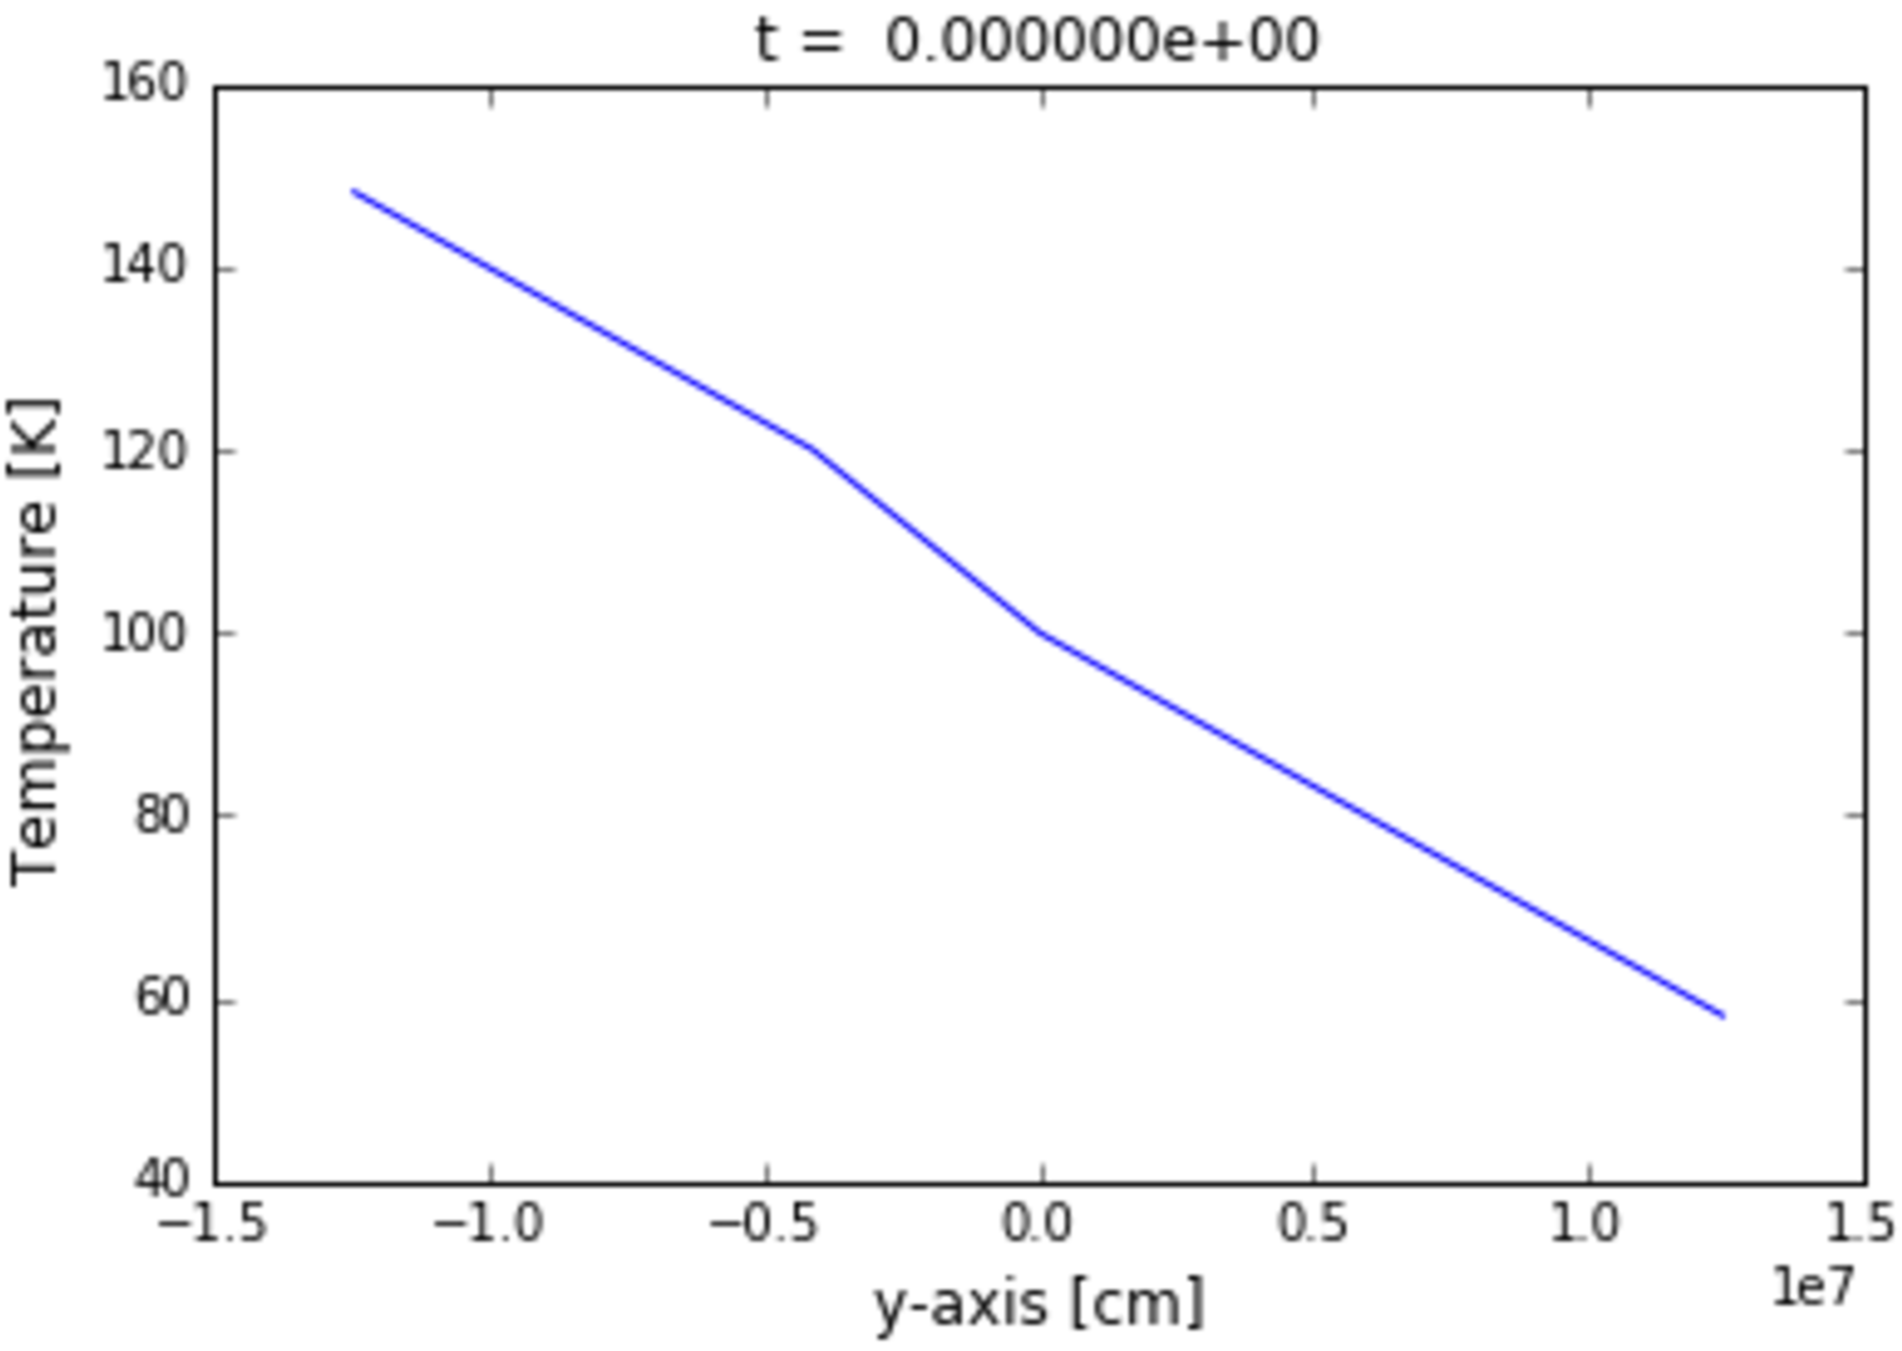
\includegraphics[width=10cm]{tempprofile}
\caption{Example of initial temperature profile along the $y$-axis}
\label{fig:tempprofile}
\centering
\end{figure}
The controlling parameter is the temperature gradient that can we initialized to any value. In our case we divided the simulated region in three parts. The bottom region (labeled as $1$) starts at the lower boundary and reaches $4/12$ of the domain, the central (labeled as $2$) proceeds till the middle, and the upper one (labeled as $3$) reaches the upper boundary, as shown in \ref{fig:tempprofile}. We define a parameter $\alpha_{i}$ ($i=1, 2, 3$) which is nothing but the fraction of the $\nabla$ over the $\nabla_{\mathrm{ad}}$. As seen in previous sections $\alpha_{i}<1$ implies stability in the $i-$region, instability otherwise. \\
\begin{figure}[t]
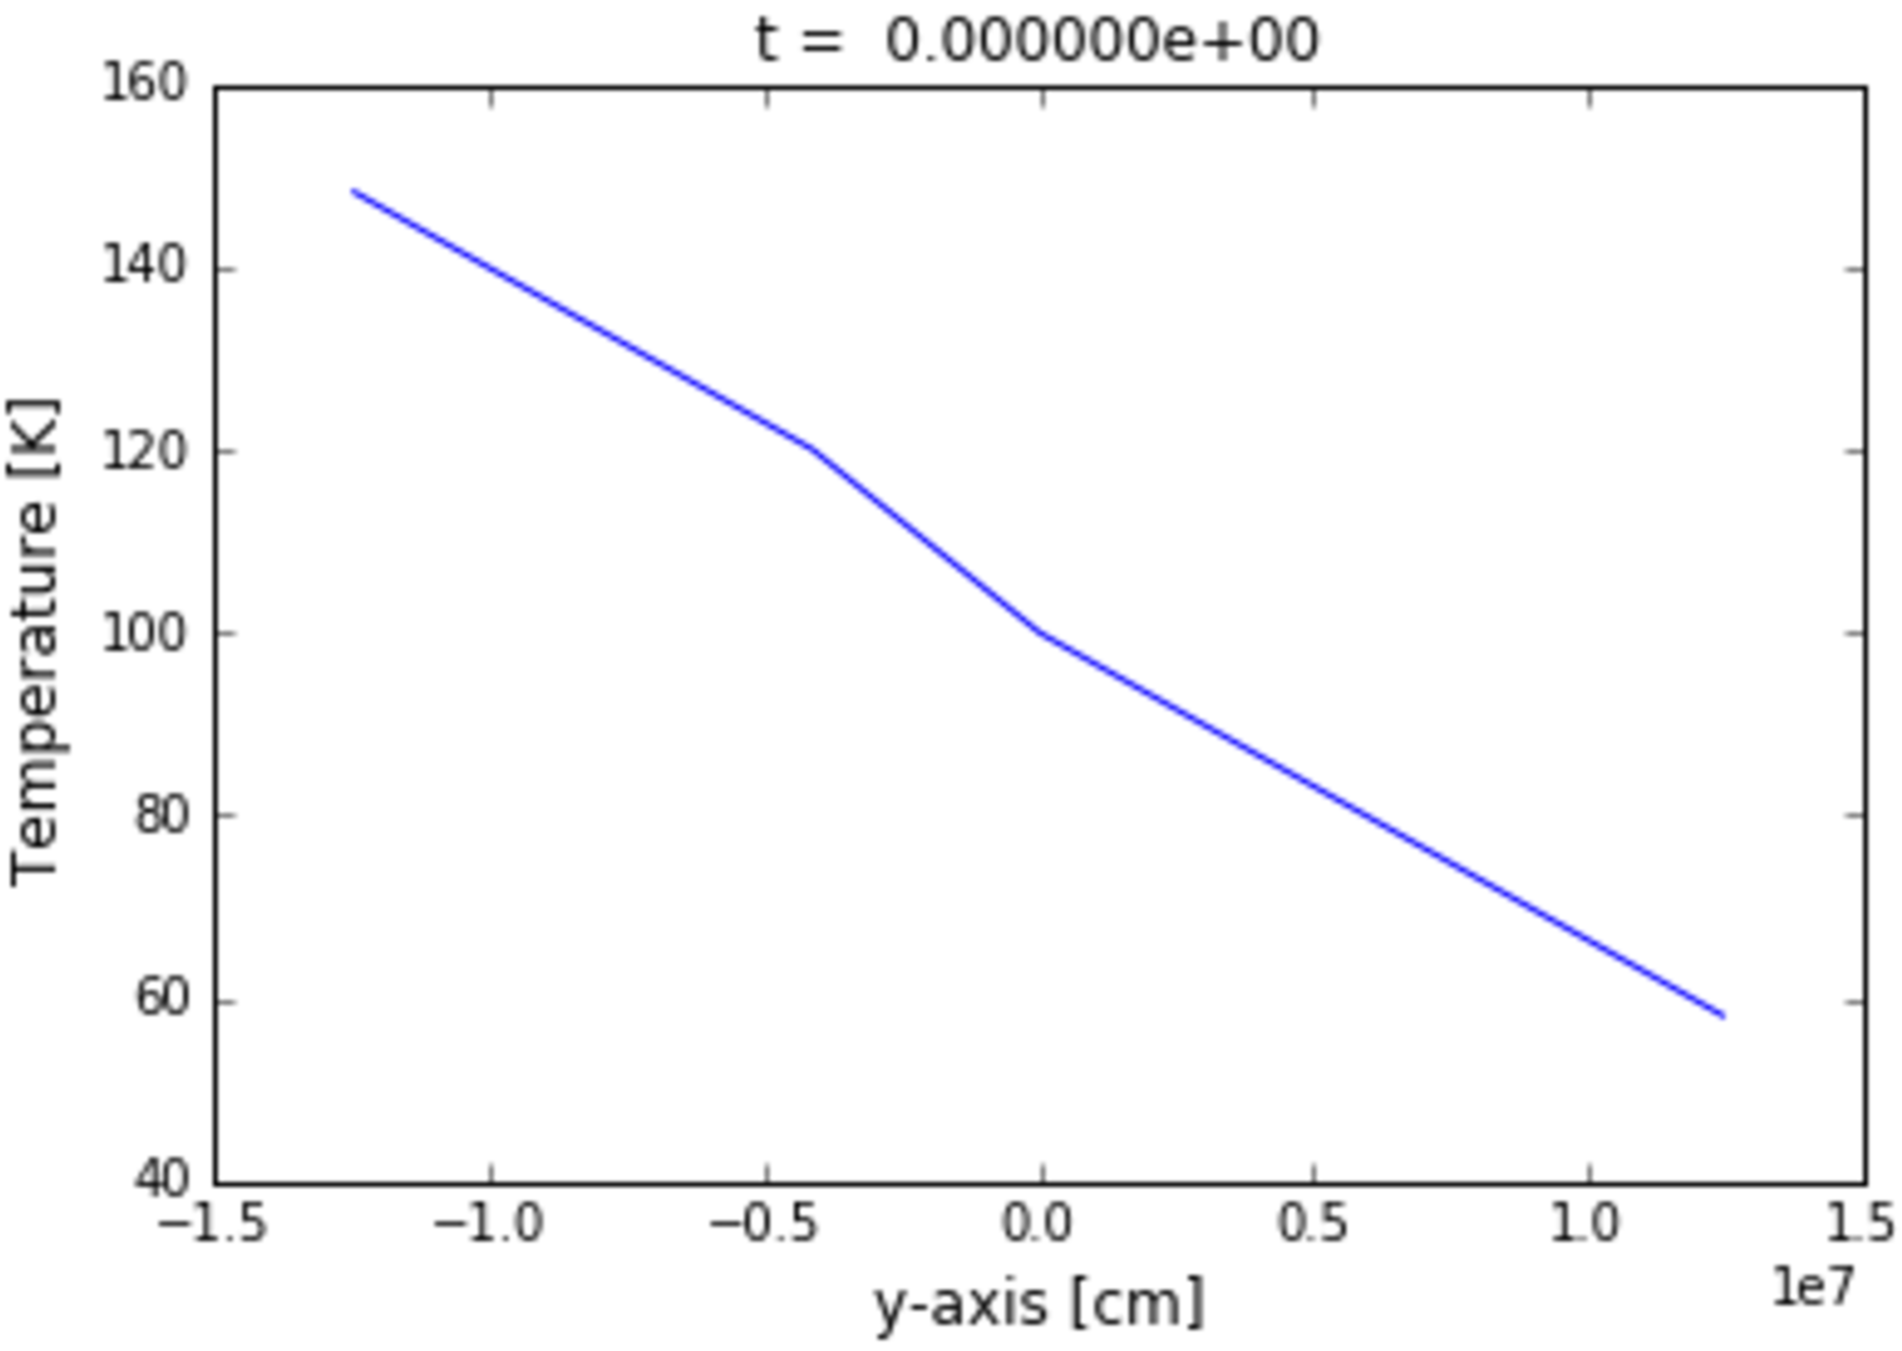
\includegraphics[width=10cm]{tempprofile}
\caption{Example of initial temperature profile along the $y$-axis}
\label{fig:tempprofile}
\centering
\end{figure}
We always initialized the setup with $\alpha_{1} = \alpha_{3}$ widely smaller than $1$; and $\alpha_{2}=0.99$, which means a very precarious situation in terms of stability in the second region. A heating function furthermore heats the second region with a gaussian profile (see \label{fig:tempprofile}) to generate convection that will expand downward and upward by accretion. The values of $\alpha_{1}$ and $\alpha_{3}$ are controlling parameters for the bulk-Richardson number, since they are proportional to $\Delta b$. The advantage of simulating a strip of convection between two stable layers (miming a Shell convection) instead of a convective region at the bottom that grows upward (Core convection-like) is twofold: it gives us two convective boundaries to study instead of one, and we avoid high mach number at the boundary which can at times generate problems or unphysical situations. \\
One of the hardest tasks has been to generate the correct amount of heating such that the turbulence route mean square \textit{at the interface} was constant during the run (which is one one of the ingredients of the bulk-Richardson number, hence one of the parameters we want to control in order to perform a differential study). The heating function also checks at every time step if in any cell of the grid a given mach number limit is reached. In that case the total heating is reduced to $50 \%$ of the original amount.\\ 
At the bottom of the simulated region small perturbations in temperature and mach number had been imprinted on the stratification in order to break the initial symmetry of the system.\\
A wide range of boundary condition has been tested for this problem. Periodic boundaries along the $y$-axis would have provided the most physical solution, unfortunately an horizontal shear flow used to appear at the onset of convection. We observed the same shear flow using boundary with constant extrapolation for the velocity field. Eventually we decided to use wall boundary conditions everywhere. \\
As briefly explained in the previous sections, in order to define the topology of the convective boundaries, we injected a passive scalar inside the central region. Recall that passive scalars are just like colors of the fluid and in no way they influence the dynamic of the system, neither they diffuse.\\
As previously stated our goal is to perform a \textit{differential} study of the bulk-richardson number and the CBM problem. This implies running simulations with different values of $\Delta b$ and $\sigma_t$ at different resolutions. Being 2D simulations computationally speaking so cheap we managed to run a copious amount of them. As reported in ??? we run with $\alpha_1=\alpha_3=0.2, 0.7$, mach number limit of $0.5, 0.01$, and resolution spanning from $256 \times 128$ (Low Resolution, LR), $512 \times 256$ (MR), $1024 \times 512$ (HR), $2048 \times 1024$ (VR). With this notation with the code 2d0.7-0.01HR we refer to a 2 dimensional simulation, with $\alpha_1=\alpha_3=0.7$, a reduction of the heating at mach $0.01$ on a $1024 \times 512$ grid. \\
It is worth noticing that a higher resolution in CFD does not only mean resolving better the system, but also changing the numerical viscosity of the fluid. Hence we expect to have higher mach number on higher resolution runs.
Numerical viscosity is also the reason for which on the $x$-axis the number of cells is always the double to the $y$-axis: we want to keep cells squared and not rectangular, in order to keep viscosity isotropic and prevent it from becoming a tensorial quantity. \\

\subsubsection{Evolution of a single run}
Let's consider the setup 2d0.7-0.01LR. \\
Convection starts at around $t \sim 7000 s$. Because of the already mentioned implicit time stepping, the lower the mach number, the bigger the time step, allowing us to save a huge amount of computational resources before the rise of convection. A remarkable difference is also observed in the convective regime, as long as the mach number is below $10 \%$, which will always be our case. \\
In figure \ref{fig:2d0.7-0.01LR.passive} we plot the passive scalar (initialized inside the central region) which over time is advected by convection. We clearly see the accretion of the convective boundary that over the $200000 s$ of simulated time moves gradually upward and downward. Specifically in the upper case it starts at $\sim 6.2 \times 10^{6} cm $ and ends up at $\sim 8.0 \times 10^{6} cm$, for the lower case it starts at $\sim 3.7 \times 10^{6} cm$ and moves downwards to $\sim 3.1 \times 10^{6} cm$. \\
In figure \ref{fig:2d0.7-0.01LR.mach} we plot profile of the mach number over the simulated time. It is what one would expect by looking at the passive scalar adcevtion, with two remarks that need to be done. \\
First of all the mach number slightly grows over time but not dramaticaly, thanks to the heating function that we implemented, featuring a cutoff as previously explained. \\
Second of all it is clear that some internal modes are excited by the convective blobs when they hit the stable layers and they propagate through it. They appear more significative in the upper region and to a certain extent it's true, but mainly this is due to the fact that the speed of sound there it's lower. Plotting the absolute velocity the difference is not so dramatic. An intresting question why will try to answer to is obviously to which extent these internal modes influence the dynamic of the boundary. \\
\begin{figure}[t]
  \centering
    \subfloat[Advection of passive scalar and convective boundary growth]{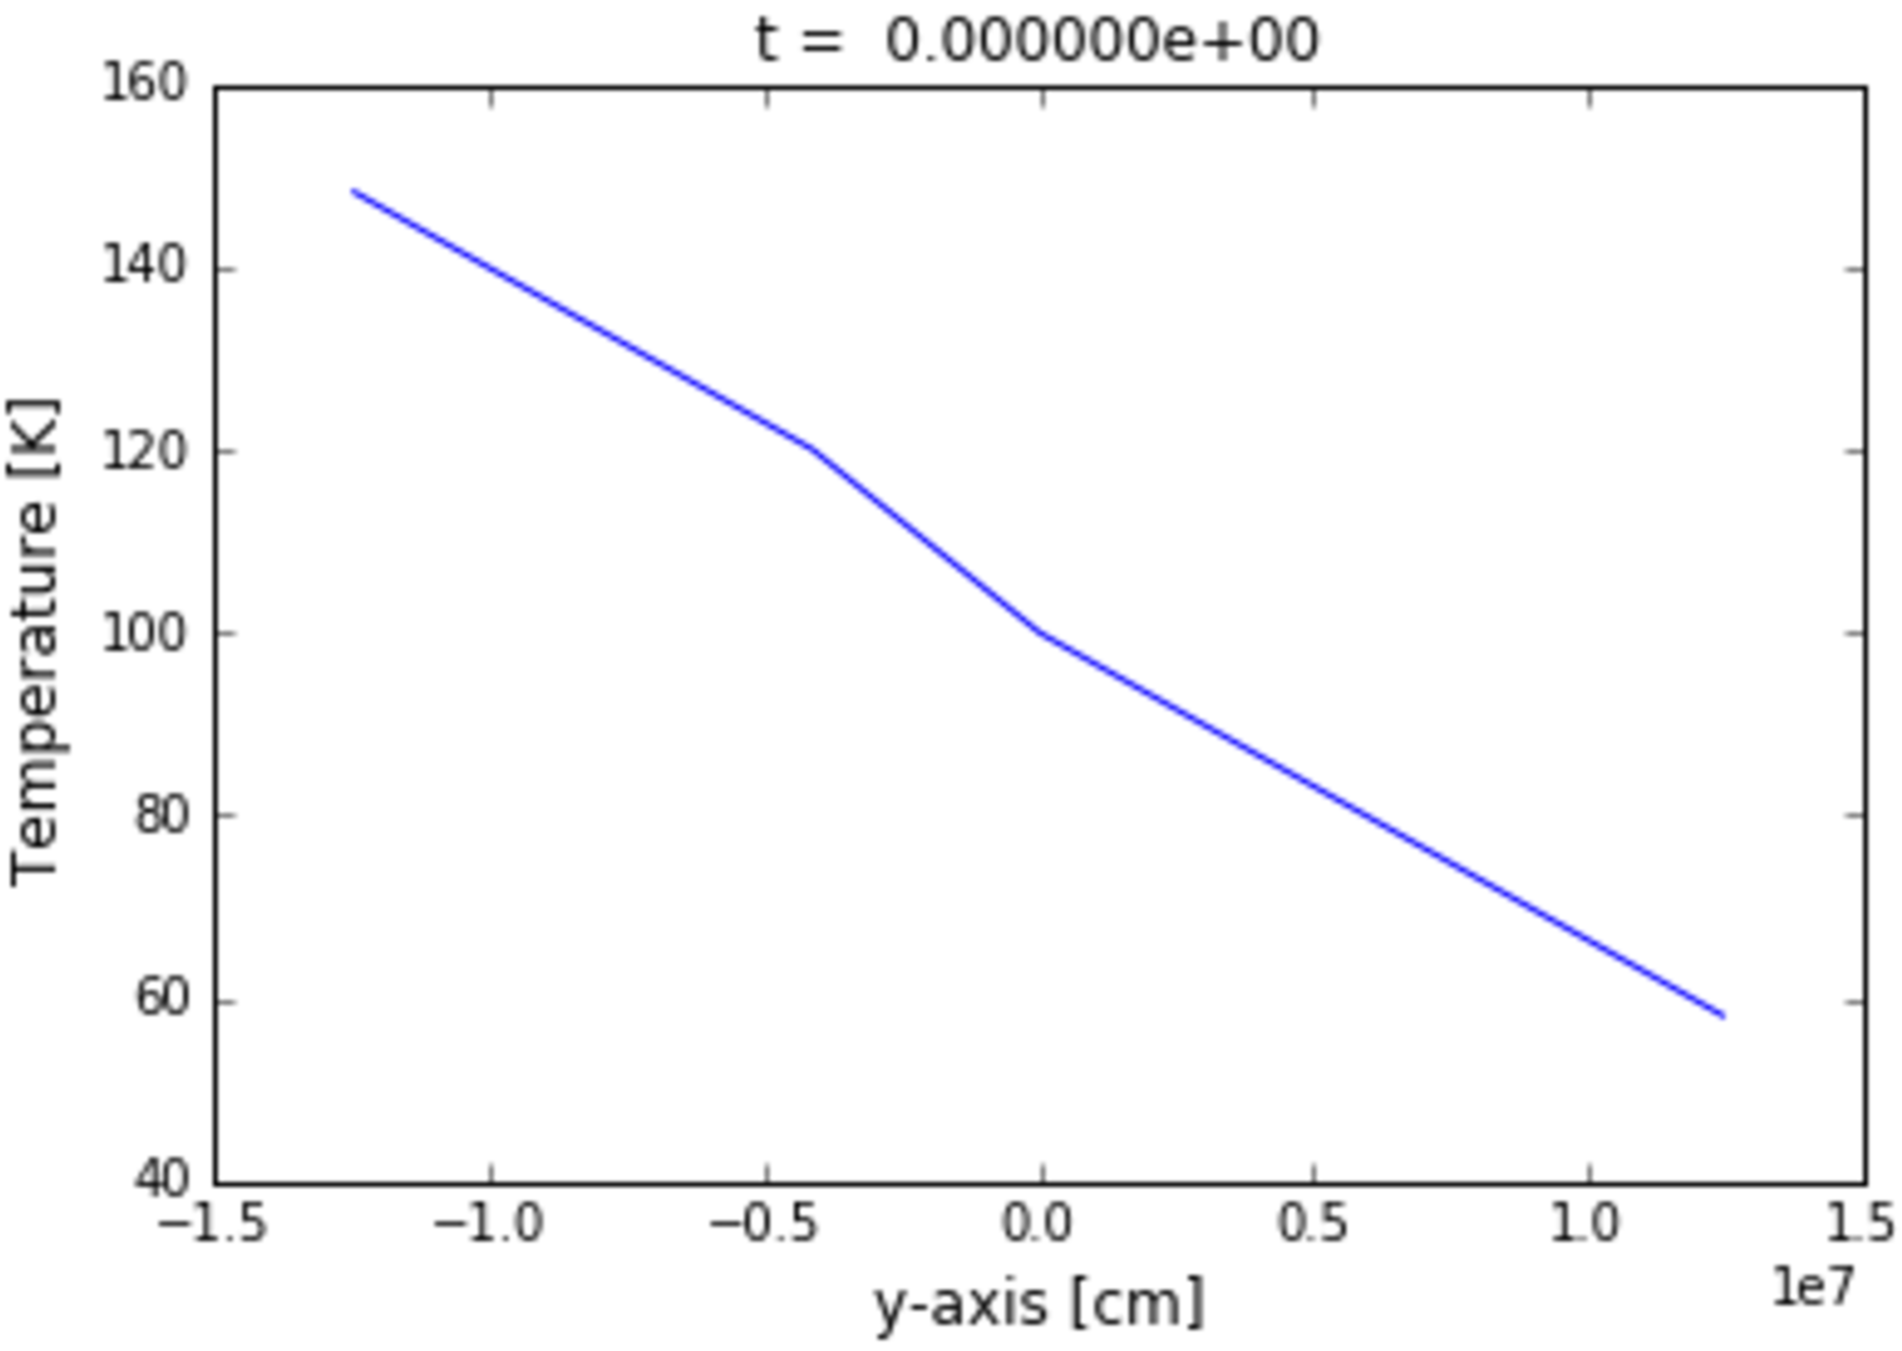
\includegraphics[width=0.4\textwidth]{tempprofile}\label{fig:2d0.7-0.01LR.passive}}
      \hfill
        \subfloat[Profile of the mach number over time]{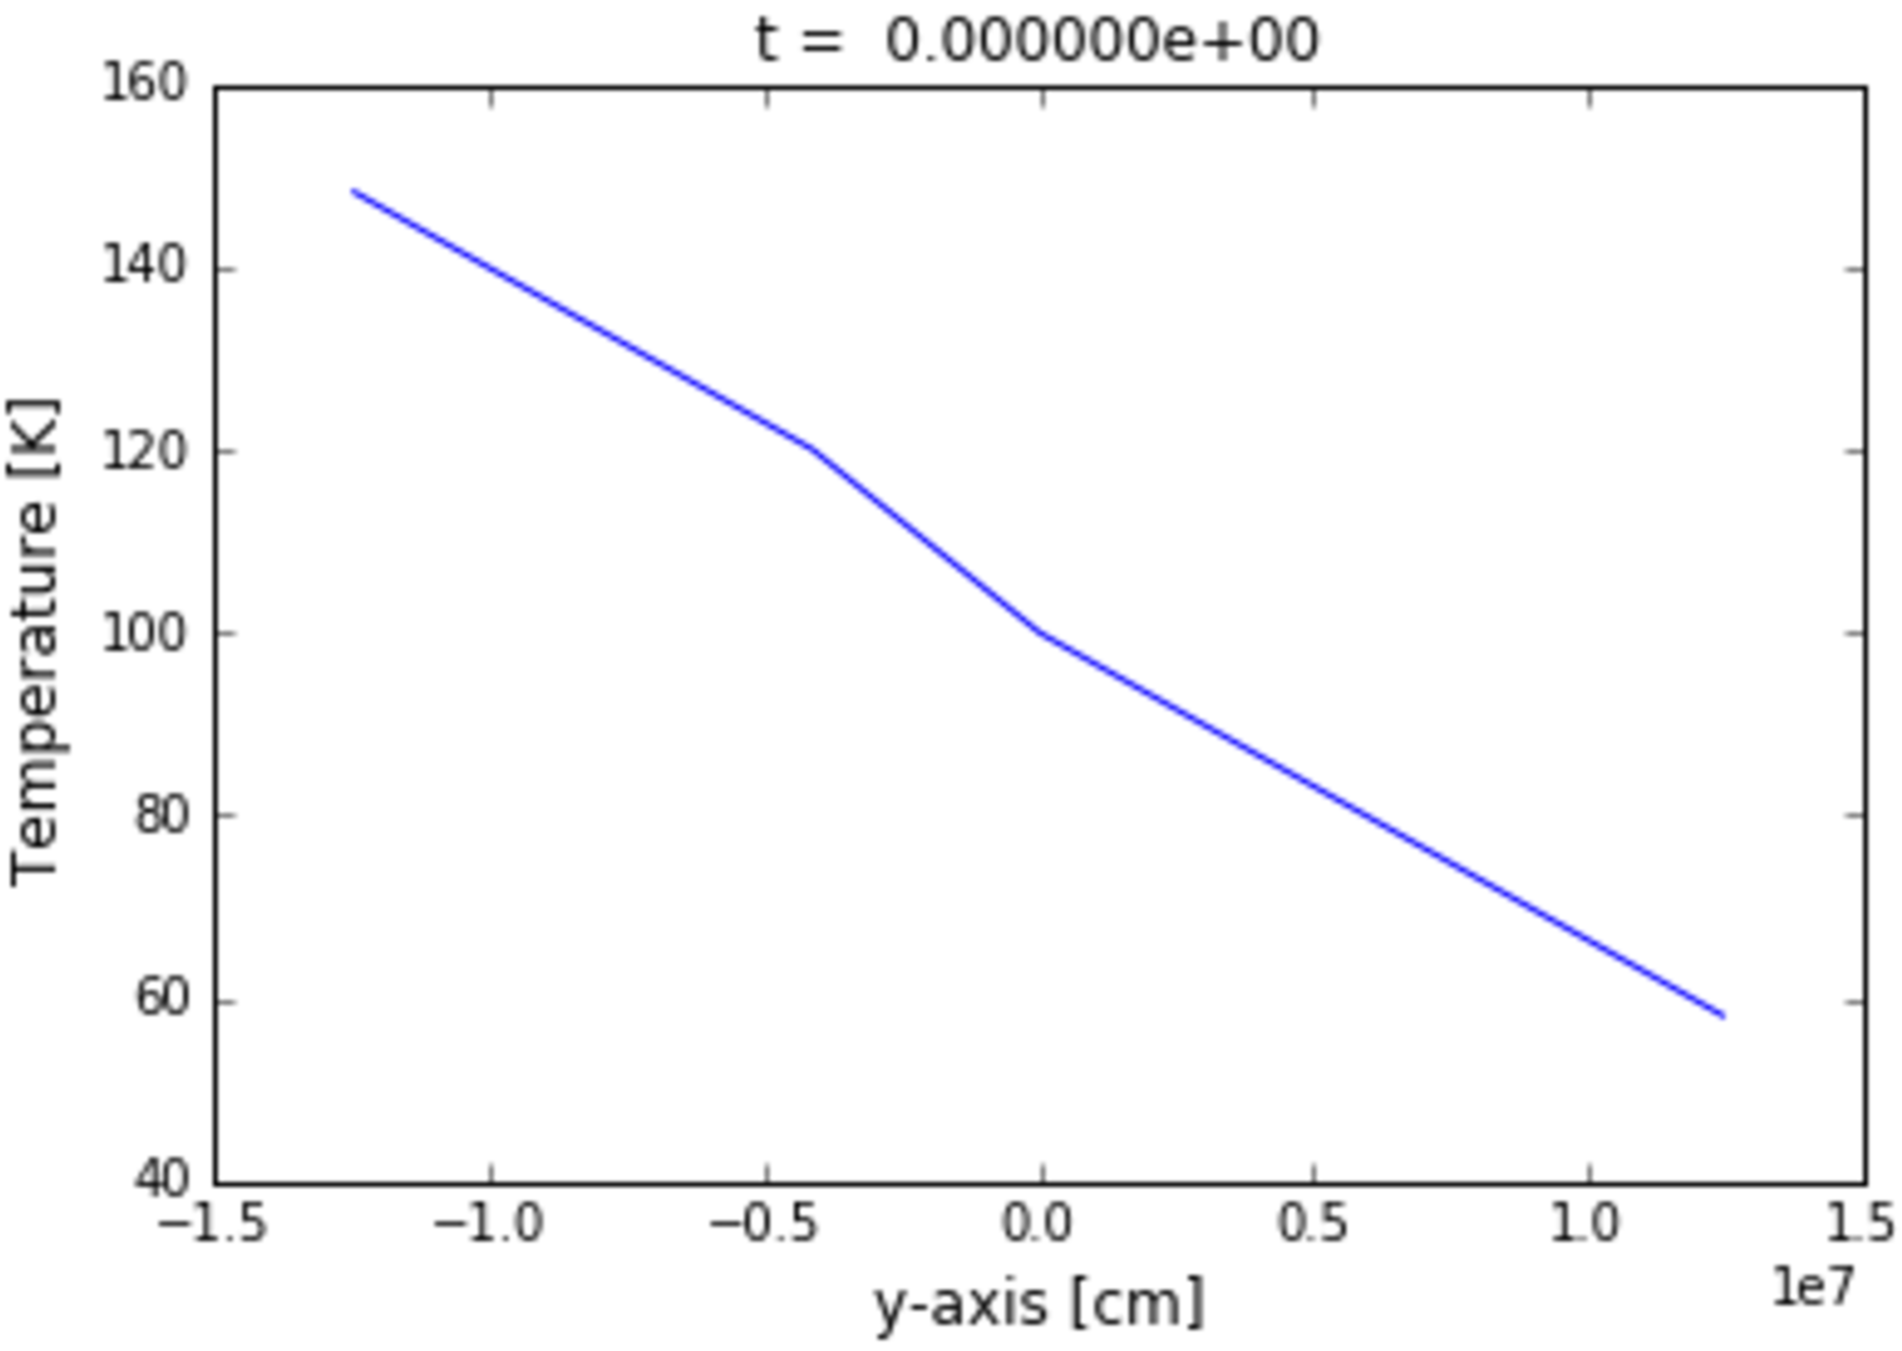
\includegraphics[width=0.4\textwidth]{tempprofile}\label{fig:2d0.7-0.01LR.mach}}
	  \label{2d0.7-0.01LR.passive}
  \end{figure}
In figure \ref{fig:2d0.7-0.01LR.bp} we plot the parameters needed to compute the bulk-Richardson number for the upper boundary. \\
We show first of all the boundary position over time with its rms. It's clear that after $t \sim 100000 s$ there is a slow down, and we suspect that this is due to the interaction with the internal modes. \\
Second of all we plot in figure \ref{fig:2d0.7-0.01LR.turbmach} the turbulence rms mach number at the interface. This is not constant over the run, instead it oscillates, but we are satisfied by the fact that it remains in the same order of magnitude. There is also a tiny trend to increase, but as previously stated, it is an extremely hard task to tune the heating in order to obtain a perfectly constant turbulent regime. \\
\begin{figure}[t]
  \centering
    \subfloat[Advection of passive scalar and convective boundary growth]{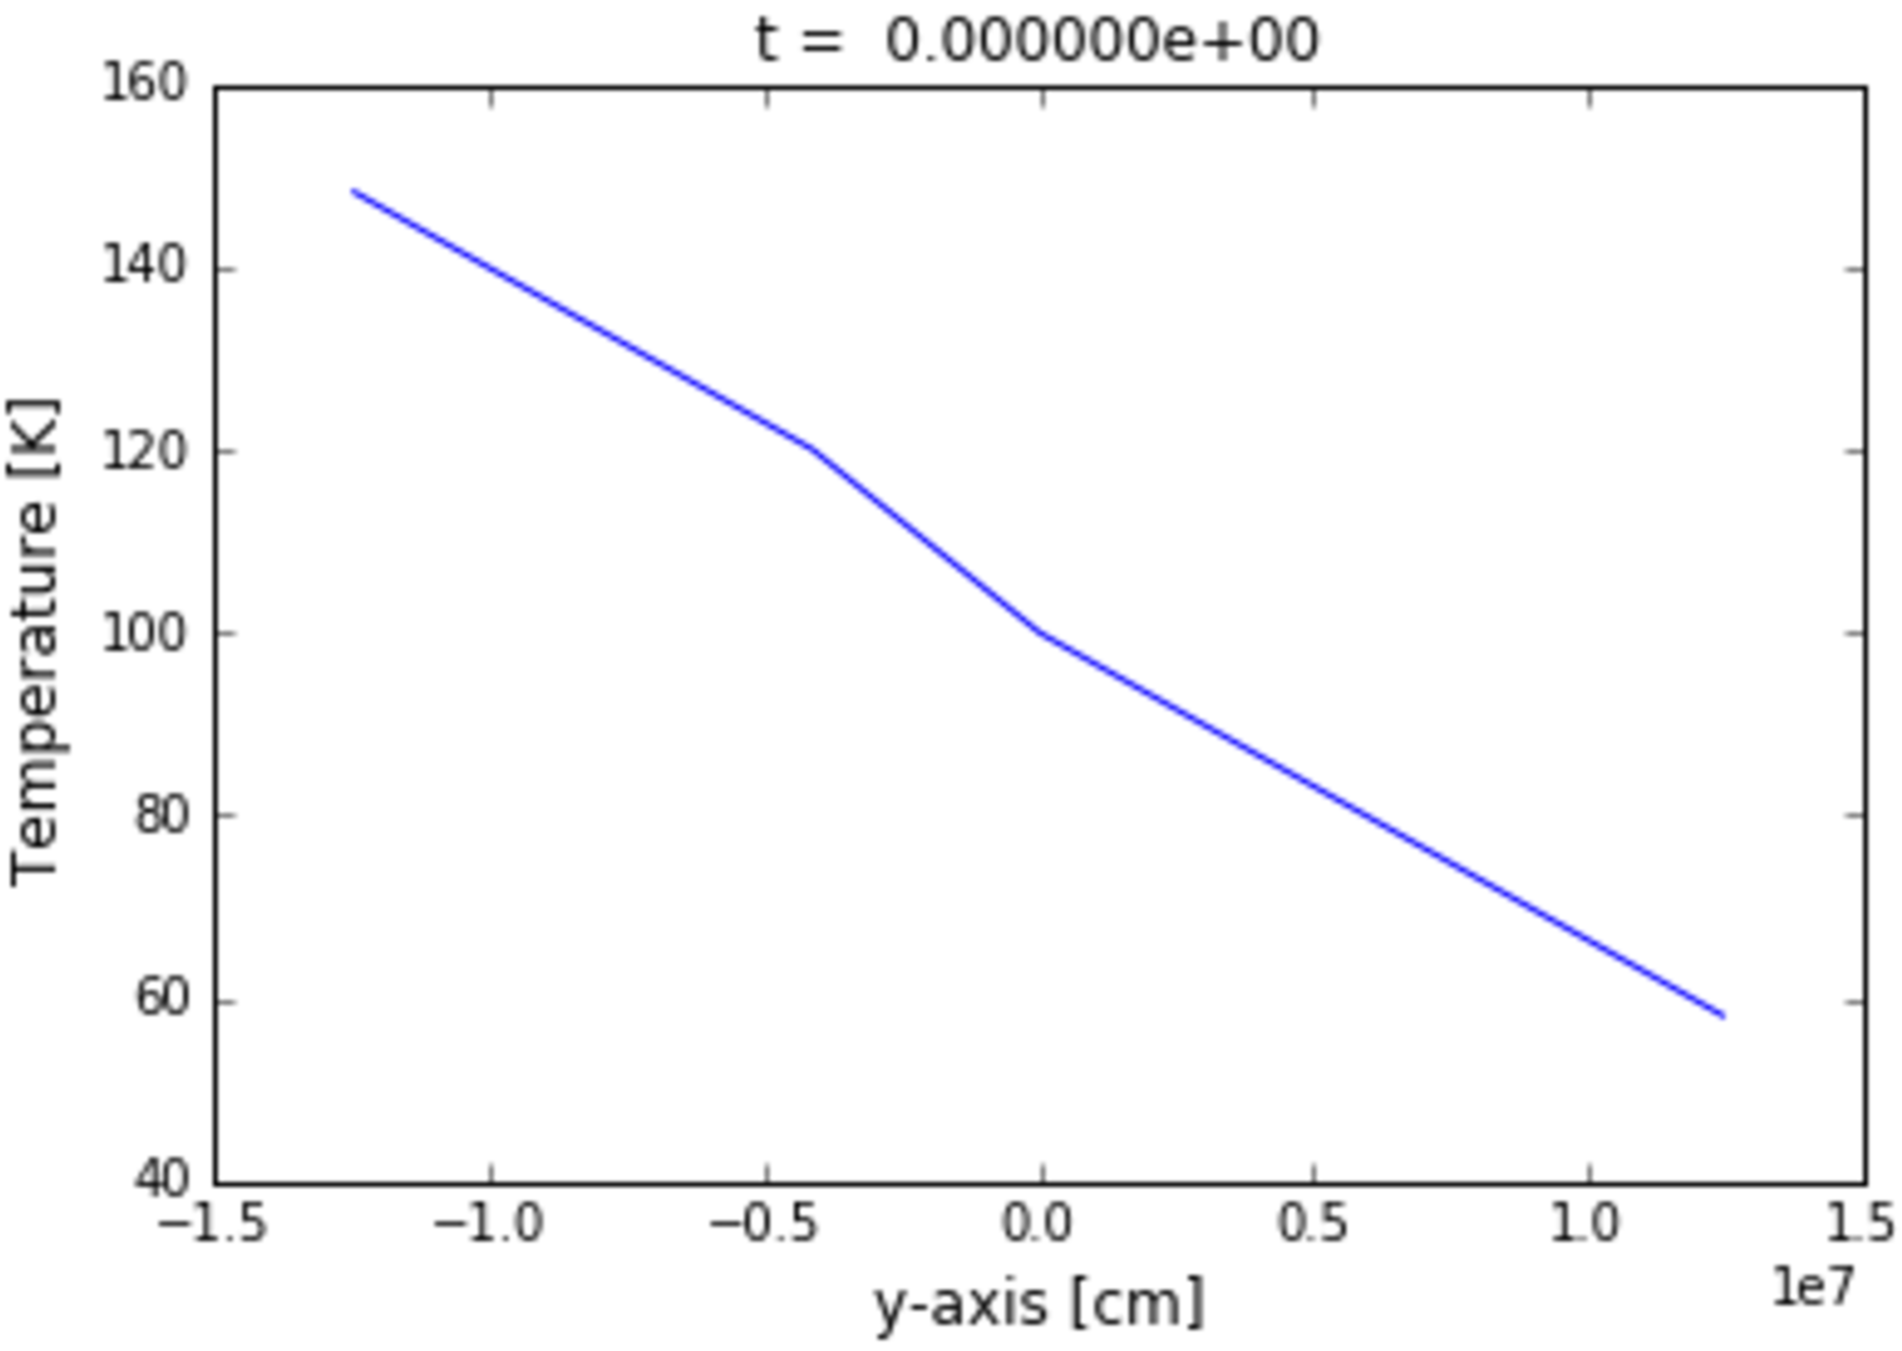
\includegraphics[width=0.4\textwidth]{tempprofile}\label{fig:2d0.7-0.01LR.bp}}
      \hfill
        \subfloat[Profile of the mach number over time]{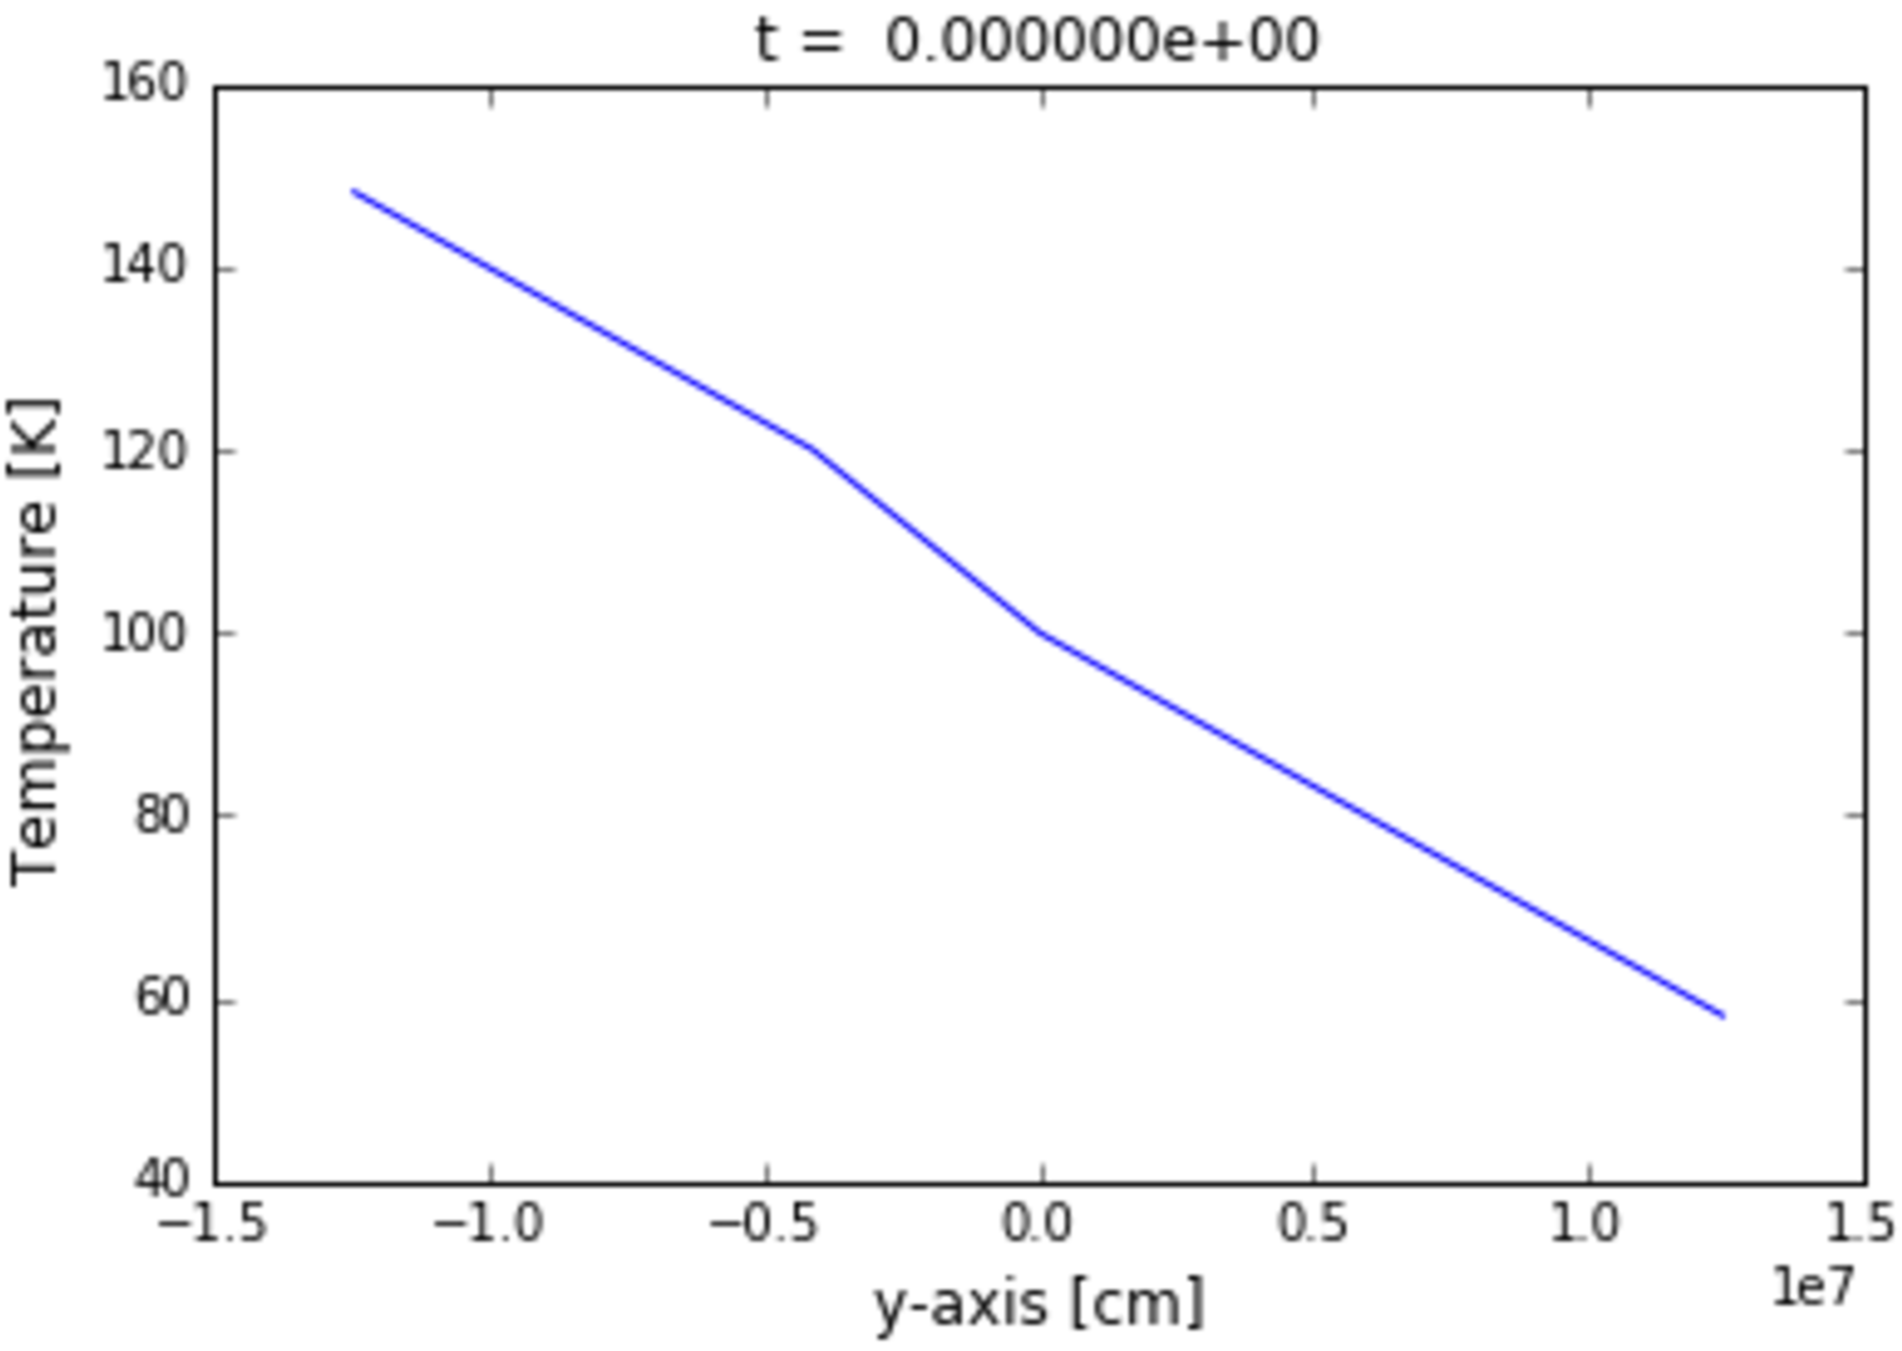
\includegraphics[width=0.4\textwidth]{tempprofile}\label{fig:2d0.7-0.01LR.turbmach}}
      \hfill
        \subfloat[Profile of the mach number over time]{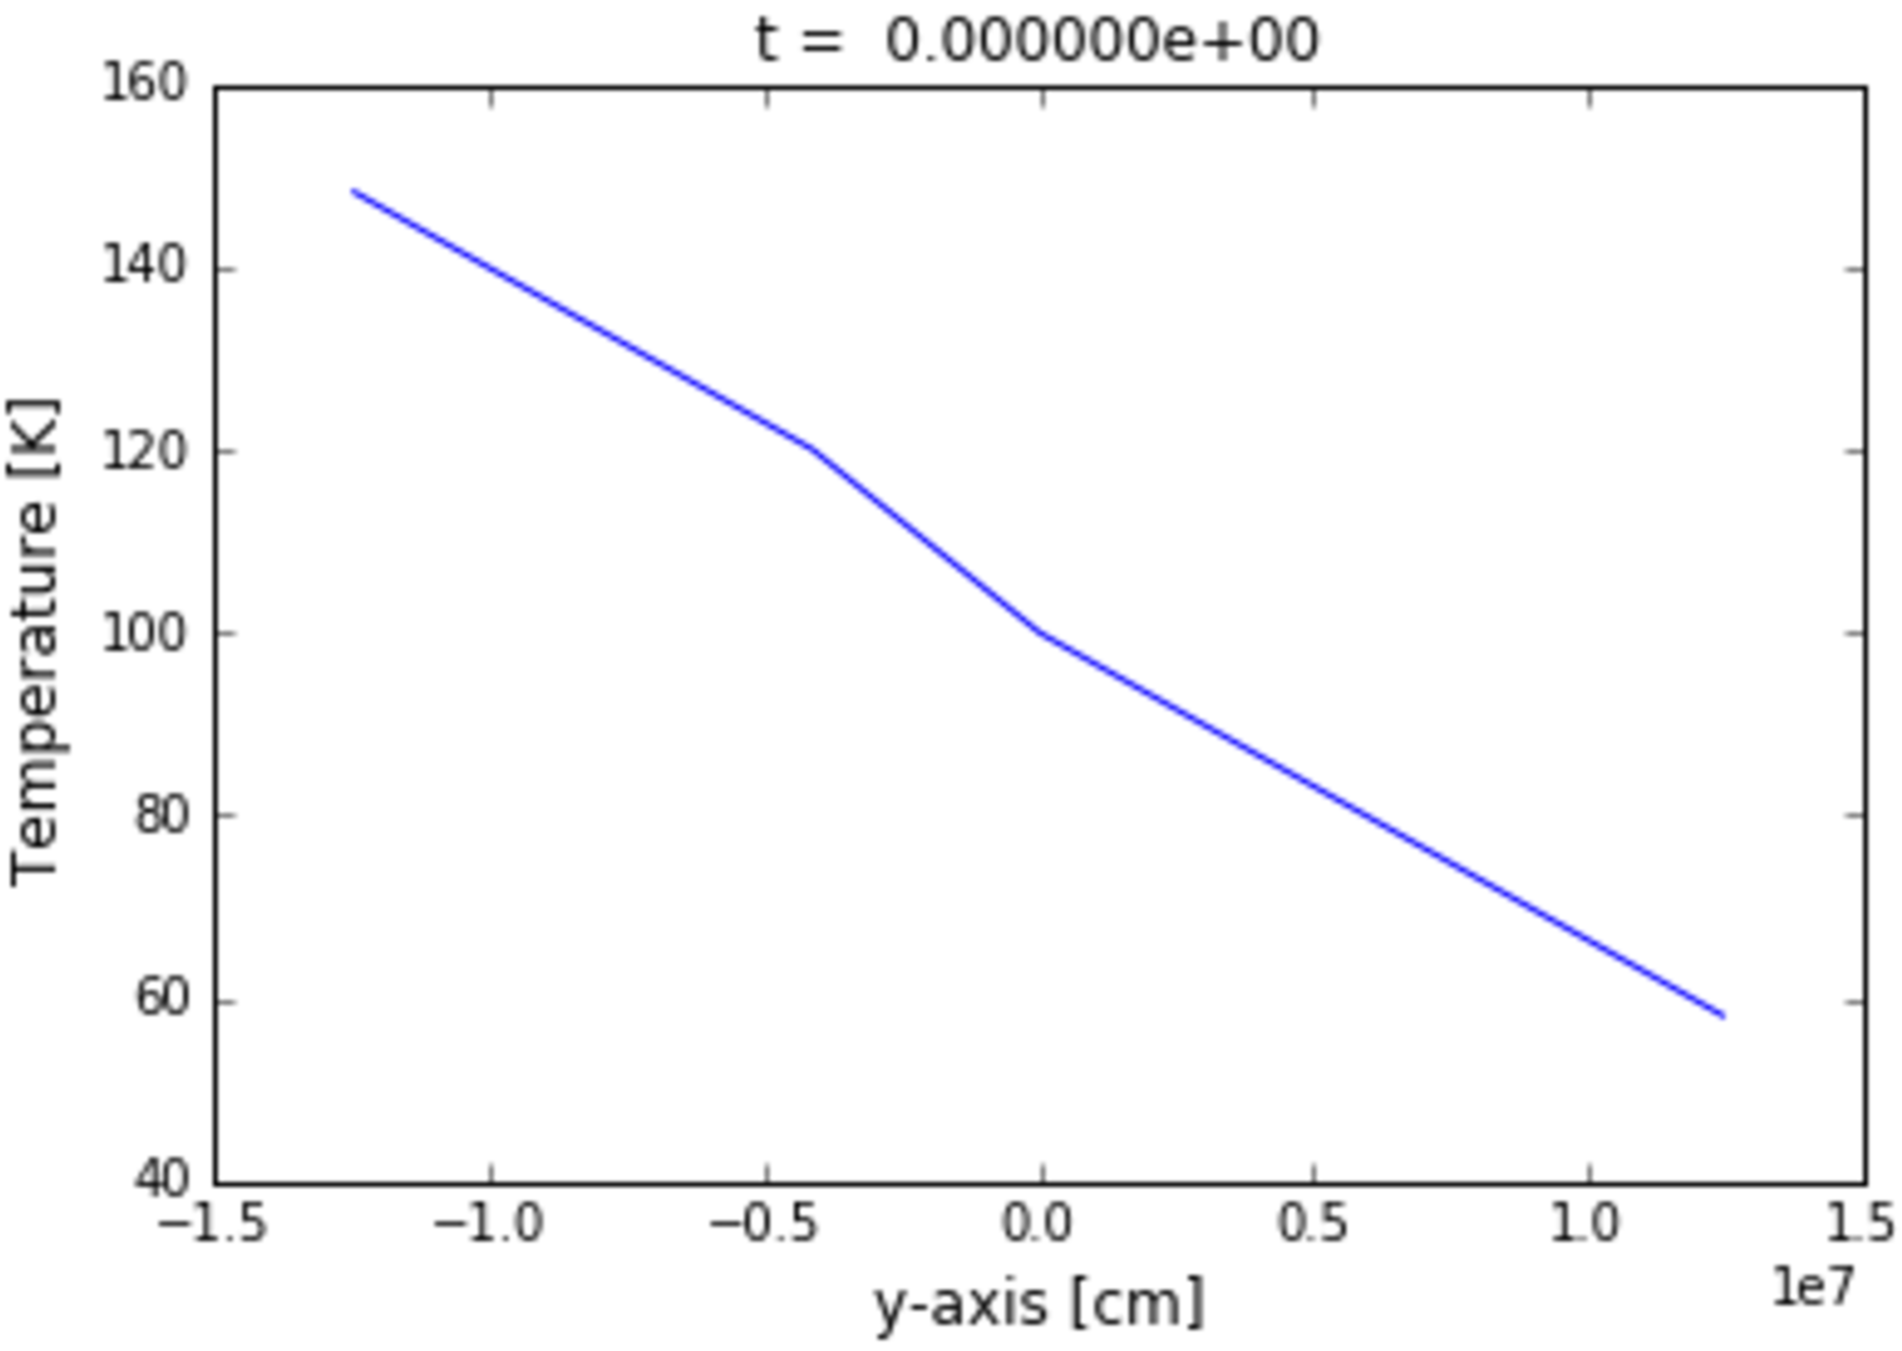
\includegraphics[width=0.4\textwidth]{tempprofile}\label{fig:2d0.7-0.01LR.delb}}
      \hfill
        \subfloat[Profile of the mach number over time]{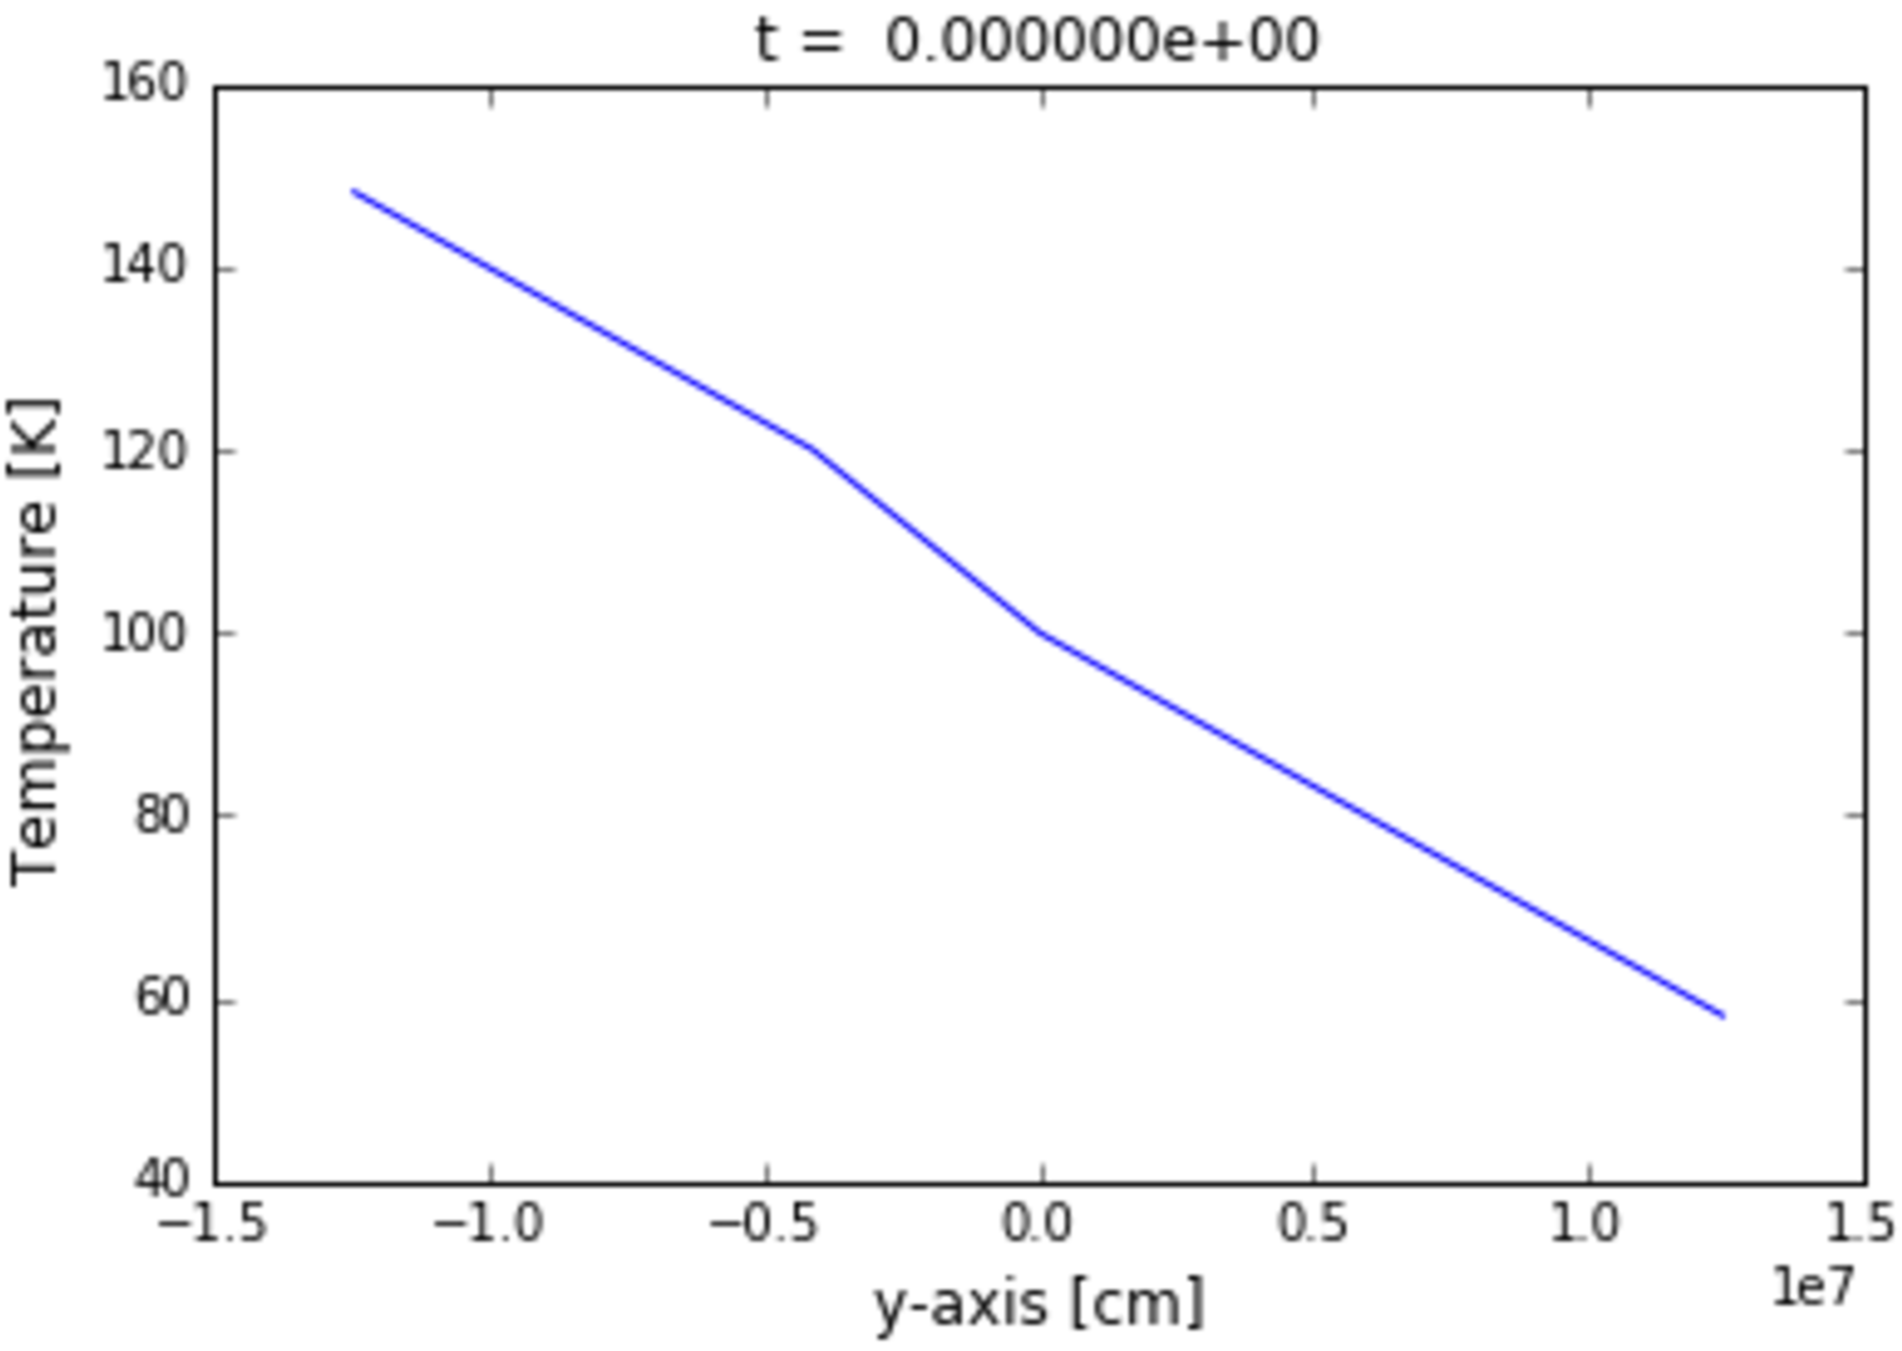
\includegraphics[width=0.4\textwidth]{tempprofile}\label{fig:2d0.7-0.01LR.l}}
	\caption{prova caption}
  \end{figure}
In figure \ref{fig:2d0.7-0.01LR.delb} we plot the buoyancy jump acros the interface. By looking at this it is clear that the resolution used in this run is absolutely not enough to properly resolve the system. As previously explained the $\Delta b$ is obtained by integrating the Brunt-Väsälä frequency over the boundary rms, but in some cases this is less than half of a cell, hence when discretized it goes down to zero. This is the reason for which we get a plot with such discontinuities. As we will see, this inconvenient will not occur anymore with higher resolution runs. \\
Last we plot in figure \ref{fig:2d0.7-0.01LR.l} the turbulence length scale. This is computed by autocorrelating the mach number at the center of the convective region, and then taking the length at which the autocorrelation function drops below $0.5$. It is remarkable that this parameter oscillates very much over a full order of magnitude, but does not show any increasing or decreasing trend. We decided to compute it in the middle of the region, rather than on the boundary, because in the second case the magnitude of the oscillation was too high and impracticable. \\
For every 2D or 3D run we will extrapolate the relevant parameters and present in the following layout
\begin{center}
 \begin{tabular}{|l|c|c|c|c|c|c|}
	  \hline
	  Run & $\Delta b$ & $\sigma_t$ & $L$ & $Ri_{\mathrm{B}}$ & $u_E$ & exp vel\\
	  	\hline
		2d0.7-0.01LR & 5 & 7& 5 & 7& 5 & 7 \\ 
	      \hline
      \end{tabular}
 \end{center}

\subsubsection{Resolution study}
The previous LR case is the lowest resolution we can use to compute the buoyancy jump. The reason is that when using a $128 \times 64$ grid, the boundary width is at times below half of a cell (which is consequentially rounded down to zero), leading to $\Delta b =0$. Once the resolution is enhanced at the point that the bouyancy jump is always nonzero, still this does not imply that we are properly resolving all the features of the system relevant to our problem, like smaller turbulent blobs that might have an impact on the CBM. For this reason we run the previous setup at different resolution, and we are going to discuss the results in the following paragraphs.


  %%%%%%%%%%%%%%%%%%%%%%%%%%%%%%%%%%%%%%%%%%%%%%%%%%%
% SECTION CONCLUSIONS %
%%%%%%%%%%%%%%%%%%%%%%%%%%%%%%%%%%%%%%%%%%%%%%%%%%%%%%%%%%%%%%%%%%%%%%%%%%%%%%%%%%%%%%%%%

\section{Results}
\subsection{ciao}
ciao
\end{document}
